\documentclass[sigconf,table]{acmart} 
%\settopmatter{printacmref=false} % Removes citation information below abstract
%\renewcommand\footnotetextcopyrightpermission[1]{} % removes footnote with conference information in first column
% \pagestyle{plain} % removes running headers
%\fancyfoot{} % for removing "manuscript submitted to ACM" running footer

%\bibliographystyle{plainurl}

% packages
\usepackage{amsmath}
\usepackage{amsfonts}
\usepackage{amssymb}
\usepackage{xcolor}
\usepackage{enumerate}
%\usepackage{enumitem}
\usepackage{paralist}
%\usepackage{amsthm}
\usepackage{algorithm}
\usepackage{algpseudocode}
\usepackage{graphicx}

% comment macros
\newcommand{\KM}[1]{{\color{red} \textbf{KM:} #1}}
\newcommand{\MS}[1]{{\color{blue} \textbf{MS:} #1}}
\newcommand{\MZ}[1]{{\color{green} \textbf{MZ:} #1}}

% macros
\newcommand{\Sol}{\mathit{Sol}}
\newcommand{\Xh}{\widehat{X}}
\newcommand{\xh}{\widehat{x}}
\newcommand{\Uh}{\widehat{U}}
\newcommand{\fh}{\widehat{f}}
\newcommand{\Beh}{\mathcal{B}}
\newcommand{\nom}{\mathit{nom}}
\newcommand{\reach}{\mathit{Reach}}
\newcommand{\avoid}{\mathit{Avoid}}
\newcommand{\bound}{\mathit{Domain}}
\newcommand{\set}[1]{\{ #1 \}}
\newcommand{\frr}[1]{\preceq_{#1}}
\newcommand{\ol}{\mathrm{OL}}
\newcommand{\cl}{\mathrm{CL}}
\newcommand{\findAbs}{\mathit{ComputeAbstraction}}
\newcommand{\ball}{\Omega}
\newcommand{\obs}{\mathit{obs}}
\newcommand{\col}{\mathit{col}}
\def\reals{\mathbb{R}}
\def\ints{\mathbb{Z}}


% environments
\newtheorem{subproblem}{Subproblem} % for the packages and the macros

%\title{Multi-Agent Reach-Avoid Control with Formal Guarantees}

\title{Symbolic Reach-Avoid Control of Multi-Agent Systems}
%\author{Mehrdad, Kaushik, Mahmoud, Rupak, Sadegh}

\author{Rupak Majumdar} 
\orcid{https://orcid.org/0000-0003-2136-0542}
\affiliation{MPI-SWS, Germany.}
 \email{rupak@mpi-sws.org} 
 
 \author{Kaushik Mallik} 
 \orcid{https://orcid.org/0000-0001-9864-7475} 
 \affiliation{MPI-SWS, Germany.} 
 \email{kmallik@mpi-sws.org} 

 \author{Mahmoud Salamati} 
 \orcid{https://orcid.org/0000-0003-3790-3935} 
 \affiliation{MPI-SWS, Germany.} 
 \email{msalamati@mpi-sws.org} 
 
 \author{Sadegh Soudjani} 
 \orcid{https://orcid.org/0000-0003-1922-6678} 
 \affiliation{Newcastle University, UK.} 
 \email{sadegh.soudjani@ncl.ac.uk}
 
  \author{Mehrdad Zareian} 
 \orcid{https://orcid.org/0000-0001-7421-0850} 
 \affiliation{MPI-SWS, Germany.} 
 \email{mzareian@mpi-sws.org} 

\makeatletter
% \@ifclassloaded{acmart}{\keywords{Abstraction Based Controller Design, Tracking Control}}{}
\makeatother

% copyright info
\acmYear{2021}\copyrightyear{2021}
\setcopyright{rightsretained}
\acmConference[ICCPS '21]{ACM/IEEE 12th International Conference on Cyber-Physical Systems (with CPS-IoT Week 2021)}{May 19--21, 2021}{Nashville, TN, USA}
\acmBooktitle{ACM/IEEE 12th International Conference on Cyber-Physical Systems (with CPS-IoT Week 2021) (ICCPS '21), May 19--21, 2021, Nashville, TN, USA}
\acmPrice{}
\acmDOI{10.1145/3450267.3450548}
\acmISBN{978-1-4503-8353-0/21/05}

% CCS
\begin{CCSXML}
<ccs2012>
   <concept>
       <concept_id>10010520.10010553.10010554.10010556</concept_id>
       <concept_desc>Computer systems organization~Robotic control</concept_desc>
       <concept_significance>500</concept_significance>
       </concept>
 </ccs2012>
\end{CCSXML}

\ccsdesc[500]{Computer systems organization~Robotic control}


\sloppy

\begin{document}


\begin{abstract}
	%! TEX ROOT = ./main.tex

We consider the decentralized controller synthesis problem for multi-agent control systems for joint reach-avoid specifications.
Each control system is modeled as a nonlinear dynamical system with disturbance, the control objective is to synthesize \emph{local}
feedback controllers that guarantee that the overall system meets the specification even under the influence of disturbances.
%
Existing techniques based on planning or trajectory optimization usually ignore the effects of disturbance and produce open-loop
\emph{nominal} trajectories which may not suffice in the presence of disturbances.
Techniques based on formal synthesis of temporal controllers do not scale as the number of agents increase.

We propose a two-level solution approach that combines fast global nominal trajectory generation and local application of formal synthesis.
At the top level, we ignore the effect of disturbances and obtain a joint open-loop plan for the system using a fast trajectory optimizer.
At the lower level, we use abstraction-based controller design to synthesize a set of decentralized feedback controllers 
that track the high level plan against worst-case disturbances.
We demonstrate the effectiveness of our approach on several multi-robot examples using two particular classes of control specifications.
In the first type, we assume that the robots need to fulfill their own reach-avoid tasks while avoiding collision with the other robots.
In the second type, we require the robots to fulfill reach-avoid tasks while maintaining certain formation constraints.
Our experiments show that the combination technique is able to produce formally guaranteed feedback controllers while scaling to many robots.
In contrast, nominal open loop controllers did not guarantee the property and formal synthesis approaches did not finish.

\end{abstract}

\maketitle

%! TEX ROOT = ./main.tex

\section{Introduction}

Synthesizing formally verified controllers for safety-critical dynamical systems has emerged as an important problem.
The goal is to algorithmically synthesize controllers so that the systems under control only do what they are meant to do, even in the presence of external disturbances.
One such algorithmic technique is the so-called Abstraction-Based Controller Design (ABCD).
In ABCD, we start with a model of a continuous nonlinear dynamical system and a control task.
The sought controller is synthesized in three stages:
First, we approximate the continuous system model using a finite state abstraction.
Second, we compute an abstract controller for the abstraction by using reactive synthesis techniques.
Third, we refine the abstract controller to the sought final controller for the continuous system.
The desired correctness guarantee of the obtained controller follows from a careful abstraction construction process.

The strengths of ABCD are its versatility: 
It can handle arbitrary continuous nonlinear system models, external disturbances, modeling uncertainties, measurement errors, $\omega$-regular control specifications, and so on.
The weakness of ABCD is its poor scalability: 
Usually ABCD uses a state-space discretization for computing the abstraction, which causes an exponential blow-up in the time and space complexity.

In this paper, we extend ABCD---more in a practical sense---to synthesize decentralized controllers for a group of robots, operating in a shared workspace.
In general, the group can consist of a heterogeneous mix of robotic systems.
Also, we do not require the robots to be able to communicate during runtime.
We assume that each robot has been assigned a reach-avoid task, where the robot needs to reach a set of target states while avoiding a set of static obstacles.
Additionally, each robot is required to avoid collision with other (possibly moving) robots by maintaining a minimum safe distance.
We use ABCD to algorithmically come up with verified controllers for each individual robot such that all these requirements are fulfilled.

The collision avoidance requirement, in the absence of inter-robot communication, makes the controller synthesis problem especially challenging.
One option will be to treat the other robots as dynamic obstacles.
There are two problems.
Firstly, it is not known how to deal with dynamic obstacles in the ABCD framework.
Secondly, even if we knew how to deal with that, this dynamic obstacle assumption could lead to pessimistic, and often empty, solution.

On the other hand, the issue with dynamic obstacles goes away if we use a centralized approach, by treating the group of robots as one single system.
In the centralized approach, we need to build a product of the models of each individual robot; the product captures the simultaneous evolution of the global state of the system.
The states of collision, which are dynamic in nature, now conveniently become a set of static obstacles in the global state space.
We can then, at least in theory, use ABCD to synthesize a joint controller for the group of robots, and afterwards decompose the joint controller into individual controller for each robot.
(The decomposition is possible due to the underlying decentralized control structure.)

Unfortunately, ABCD does not scale to the usual large size of the global state space in the centralized approach.
To circumvent this issue, in this paper, we propose a two-layered hierarchical controller synthesis approach involving ABCD.
In the top layer, we use some off-the-shelf fast controller synthesis method to make a joint global plan using the aforementioned centralized approach.
In this paper, we use ALTRO \cite{altro} in the top layer, which is an optimal-control-based controller synthesis tool that scales quite well to large dimensional system.
Unfortunately, the fast and scalable tools, including ALTRO, usually do not provide formal guarantees against external disturbances or modeling uncertainties.
So in the bottom layer, we use ABCD to synthesize formally verified \emph{tracking} controller for each robot for following the projection of the joint plan on the robot's state space.

Our primary contribution is the extension of ABCD to tracking objectives.
This enables the use of ABCD in the hierarchical design principle, which found success in many other design contexts \cite{murray,schmidt hierarchical DES, sayan mitra}.
\todo{Need to discuss.}


\smallskip
\noindent\textbf{Related Work}
%
The field of multi-agent planning is too large for a comprehensive survey; we point to very good text books
\cite{LaValle2006,LaValle1998planning,choset2005principles,russel2010AIplanning} for an introduction.
We categorize closely related work into (1) ones combining planning and tracking controller synthesis, 
(2) ones addressing multi-agent formal controller synthesis, and 
(3) approaches combining (1) and (2).
Following are the detailed surveys of these categories:

\begin{enumerate}[(1)]
	\item Techniques combining high-level planning and low-level tracking are a staple of classical planning and control. 
More recently, several techniques consider the problem of formal guarantees for such planners.
Existing methods can be categorized based on the dynamics that they can handle (e.g., linear or nonlinear),
whether the system is subject to disturbances, considered class of specifications, and scalability. 
A common approach to solve for reach-avoid specifications is to perform the high-level planning over a lower dimensional dynamical model and then use
Sum-of-Squares (SOS) programming or Hamilton Jacobi (HJ) or satisfiabiity modulo convex programming (SMC) methods to obtain a low-level controller ensuring a bounded error between the 
two models \cite{herbert2017fastrack,DBLP:journals/corr/abs-1911-09773,singh2018robust,sun2019,Nilsson:2018}. 
\KM{Nothing has been stated about \cite{DBLP:journals/corr/abs-1911-09773,sun2019}.}
In contrast to \cite{herbert2017fastrack,singh2018robust}, our method does not require finding 
a linear mapping between the low and high dimensional models. 
Nilsson et al.  proposed a method that decomposes the state space into a lower-order planning space, and a higher-order internal dynamics space, so that planning can be performed fast and accurate tracking can be achieved using a set of control barrier functions that are computed using SOS method \cite{Nilsson:2018}. Despite providing guarantees for the worst-case bounded disturbances, their method is not capable of solving reach-avoid tasks which involve dynamic obstacles as in the multi-agent case.
%that governs the motion in planning space. 
%The planning is performed fast since it is restricted to the lower-order space. To guarantee following of the planned trajectory in the lower-order space, control barrier functions are computed using SOS method. This method, however, cannot deal with dynamic obstacles as is needed in tackling collision avoidance.}
While we choose SCOTS because the algorithm can be effectively parallelized \cite{KhaledZ19pfaces}, in principle, we could
also use SOS or Hamilton Jacobi or SMC approaches. %The existing schemes that solve the guaranteed motion planning problems in a centralized manner (e.g. \cite{sun2019}) cannot scale well.
Some other works only consider special classes of systems such as linear (\cite{fan2018controller,wongpiromsarn2012receding,Rodionova2020LearningtoFlyLC}), 
disturbance-free (\cite{tedrake2010lqr,fan2020fast,Srinivasan2018}), or finite transition systems (\cite{Yang2017milp}). 
In contrast, our method supports arbitrary 
%continuous time
 nonlinear dynamics and provides a guarantee 
against worst-case bounded disturbance.
	\item Chen et al.\ proposed a method, using control barrier functions, that requires some form of inter-robot 
communication and does not consider external disturbances \cite{Chen2018cbf}.
Sahin et al.\ proposed a method that requires the group of robots to be homogeneous \cite{Shahin2017cltl}.
There are methods which do not consider external disturbances and do not provide formal guarantees \cite{jackson2020scalable}.
	\item Alonso-Mora et al.\ proposed a method for formation control of a group of communicating homogeneous robots \cite{alonso2019distributed}.
They first synthesize nominal controller using a fast randomized geometric planning method, namely RRT, and 
then use optimal control to track the obtained nominal solution.
Unlike us, they neither consider external disturbances nor provide formal guarantees. Pant et al. considered STL expressable multi-quadrotor missions \cite{Pant2018multiquad}. They find the reference trajectory by maximizing robustness with respect to the given STL specification, and synthesize tracking controllers so that the reference trajectory is followed closely. Although their method provides some robustness margin, it is not capable of providing guarantee against worst-case bounded additive disturbances as we do. Further, they only consider time-bounded STL specifications.	
Recently, Xiao et al.\ \cite{xiao2019merging} proposed a method for synthesis of distributed controllers for a 
set of autonomous vehicles in a lane merging situation.
They use optimal control to compute a nominal controller for the product system, 
whose goal is to ensure some safety constraints together with ensuring optimality in some respect (like fuel consumption).
After that, they use control barrier functions for each robot for tracking the obtained nominal solution.
Even though they consider external noise in the system, yet, when there is noise, their controllers can 
occasionally violate the safety constraints for finite number of time steps.
Moreover, they only consider simple linear systems (double integrator) as vehicle models. 
Nikou et al. studied the problem of robust navigation for multi-agent systems \cite{Nikou2019}. 
%They consider additive bounded modelling disturbance. 
They use optimal control to compute a reference trajectory for the nominal dynamics by neglecting disturbance, and invoke a  pre-computed feedback controller to guarantee that the perturbed system's trajectory remains within a bounded hyper-cube around the reference trajectory. In order to avoid collision with obstacles or other agents, their method relies on sensing capabilities of the agents. In contrast, our method does not requires any sensing ability in order to guarantee safe navigation of multi-agents.
 %However, they assume that agents are able to communicate while moving; and their target is to satisfy input-to-state stability. In fact, their method is not able to tackle collision avoidance for static/dynamic obstacles.}

There are other works that use a pre-defined motion primitive library to perform planning for multi-robot 
systems \cite{saha2016implan,BanusicMPSZ19pgcd,Gavran2017antlab,desai2017drona}. 
In contrast, our method directly deals with the dynamical model. 
Our construction can also be seen as an \emph{assume guarantee} technique that decomposes the global problem based on nominal trajectory tubes; similar decompositions have been studied in the discrete case \cite{alur2015pattern,majumdarassume}.
The closest related work that match our level of generality is the one by Bansal et al.\ \cite{bansal2017safe}.
However, they assume that each robot has its own reach-avoid specification and they only need to avoid collision with the other robots.
In contrast, we allow global reach-avoid specifications, which subsume the specifications that they consider.
In fact, there are control problems which cannot be easily expressed in their problem setting, but can be easily expressed in our problem setting: 
examples are robots maintaining a formation while fulfilling their tasks \cite{alonso2019distributed}, etc.
\end{enumerate}

	
	%The hierarchical approach, combining high-level planning and low-level tracking, is not new.
	%Yet most of the existing works use the hierarchical approach for controller synthesis for a single robot \cite{herbert2017fastrack, fan2020fast, fan2018controller, wongpiromsarn2012receding, tedrake2010lqr, singh2018robust, DBLP:journals/tac/MeyerD19, DBLP:journals/corr/abs-1911-09773, Yang2017milp}.
	%In contrast, we consider a hierarchical control for decentralized control of a group of robots.
%	For example, there are methods which can generate nominal controlled trajectories by taking into account the maximum tracking error, assuming that a tracking controller is already in place \cite{fan2020fast, fan2018controller}.
%	On the other hand, there are methods which compute a tracking controller which minimizes the tracking error for any given nominal trajectory:
%	Some of them do not consider external disturbances \cite{tedrake2010lqr, singh2018robust}, some of them only consider linear dynamics \cite{wongpiromsarn2012receding}, and all of them consider only a single monolithic system structure \cite{herbert2017fastrack}.

% Many papers address the problem of multi-robot controller synthesis without a hierarchical approach.


% In contrast, our method can synthesize formally verified controllers for heterogeneous group of robots, subjected 
% to external disturbances, and lacking any form of communications. 
% Hierarchical controller synthesis for decentralized control of multi-robot systems is relatively rare.

% In contrast, our method provides guarantee against worst-case system noise at all time, and in addition can support nonlinear systems. 
 

%\begin{enumerate}
%	\item FastTrack: Guaranteed tracking of nonlinear trajectories for nonlinear systems under disturbances \cite{herbert2017fastrack}. \MS{They only account for the error between the planning and tracking models and not for additive disturbance applied to the tracking model. They also rely on possibility of relating the two afformentioned models by a linear mapping (which is not the case for the general class of systems). Finally, while their method scales up better than (pure) SCOTS, it does not scale up to dimensions above ten.}
%%	\item Using the tracking error in the planning phase to make sure that the controller will be safe \cite{fan2020fast}. Relies on an expert user to already provide the low-level tracking controller, whereas we synthesize the tracking controller. So they address the inverse problem in some sense.
%%	\item Another paper of the same flavor as the previous one \cite{fan2018controller}. Here they restrict themselves to discrete time perturbed linear systems.
%%	\item Sum-of-squares based tracking methods \cite{tedrake2010lqr, singh2018robust}. Do not consider external disturbances.
%	\item Other hierarchical methods using planning+tracking like approach for formal methods-based synthesis for single systems \cite{wongpiromsarn2012receding, DBLP:journals/tac/MeyerD19, DBLP:journals/corr/abs-1911-09773}.
%	
%	\item A robust scheme for controlling linear dynamical systems with additive bounded noise and (general) LTL specification \cite{Yang2017milp}. They use mixed integer linear programming (MILP) to design a nominal controller satisfying a given LTL specification in the absence of noise and then design a regulating controller to account for the noise term.
%\end{enumerate}

%\smallskip
%\noindent\textbf{Ones which address multi-robot control problems.}\
%
%\KM{The plan is to collect all the papers first in the following list. After that, I will make a story out of them.}
%Here are the papers that we know of:
%\begin{enumerate}
%	\item Safe control for multi-vehicle system under presence of disturbances \cite{bansal2017safe}. In contrast to our method, they assume a fixed priority order of the vehicles: The higher priority vehicles make independent plans, which are treated as (time-varying) obstacles for the lower priority vehicles. 
%	\new{One way our method is probably more powerful is if we consider controller synthesis for mechanically coupled systems with joint goal, or even formation control problem for mechanically decoupled systems. For these class of problems, I don't think their method will directly apply, whereas ours should work fine.}
%	
%	\item A method to control a robot swarm (modelled as planar robots with potentially different speed bounds) such that a given specification (expressable in a fragment of LTL) is satisfied \cite{Chen2018cbf}. Some extent of communication between robots is required. The collision avoidance is guaranteed via designing control barrier functions for each pair of robots. No source of disturbance is considered in the model and the proposed solution does not work for agents modeled not as planar robots.
%	\item Controlling (homogeneous) robot swarms (modelled as finite state transition systems) for satisfying specifications expressed in a temporal logic for reasoning about the collective behavior of multiple agents (cLTL) \cite{Shahin2017cltl}. Their method can potantially account for bounded noise and non-linearities, but not heterogeneity.
%	\item Controlling multi-robot (it can be heterogeneous) using ALTRO \cite{jackson2020scalable}. very similar to our work without formal guarantee but works in real-time. they are making centralized system by combining dynamics of several quads. 
%	\item The paper that we got merging example from that\cite{xiao2019merging}. They are using optimal control + control barrier function. they are can handle disturbance and in addition they are optimizing time and fuel consummation and more constraints but they are considering linear model.
%	\item Hierarchical control for interconnected discrete event systems \cite{wong1996hierarchical,schmidt2008nonblocking}.
% \end{enumerate}

%! TEX ROOT = ./main.tex

\section{Preliminaries}

%! TEX ROOT = ./main.tex

\section{The Problem Statement}
%\textcolor{blue}{
In this paper we consider planning problem for heterogeneous swarm \MZ{Swarm is not a perfect word} robotic systems with $N$  robots under the presence of model uncertainty. Each individual robot's model can be non-linear and contain bounded inaccuracy. We further assume that different robots interact each-other only through their environment and not directly. A correctly synthesized controller for a robot swarm system ensures that (1) the robot swarm reaches to its final destination in finite time, (2) the robots must not collide with each other during the execution, (3) The robots must avoid collision with static obstacles in their environment.%}

%\textcolor{blue}{%We consider planning problem for multi-robot systems modelled collectively as control system $\Sigma$ with order $n=\sum_{i=1}^N n_i$. Each of $N$ robots can be represented as a control system of order $n_i$ 
Model for each robot is given by the tuple $\Sigma^i = (X^i, U^i, W^i, f^i)$ %that consists of a state space $X^i= \reals^{n_i}$, an input space $U^i\subseteq\mathbb{R}^{m_i}$, 
%a compact disturbance set $W^i\subset \reals^{n_i}$, and 
%a function $f^i: X^i\times U^i\rightarrow X^i$ s.t. $f^i(\cdot,u^i)$ is locally Lipschitz for all $u^i\in U^i$. 
The overall \emph{control system} is represented by $\Sigma = (X, U, W, f)$ wherein $X=X^1\times X^2\times\dots\times X^N=\reals^n$, $U=U^1\times\dots\times U^N\subset \reals^m$, $W=W^1\times\dots\times W^N\subset \reals^n$ and $f=\begin{bmatrix}f^{1^T} & f^{2^T}& \dots f^{N^T}\end{bmatrix}^T$. We consider a setting wherein each individual robot starts from a (known) initial state $x_0^i\in X^i$ and is asked to go into a \emph{neighborhood} of its corresponding goal state $x_G^i\in X^i$ under the presence of non-zero disturbance. Concatenated initial and goal states of the collective swarm robot system are denoted by $x_0=\begin{bmatrix}{x_0^{1^T},\ldots,x_0^{N^T}}\end{bmatrix}$ and $x_G=\begin{bmatrix}{x_G^{1^T},\ldots,x_G^{N^T}}\end{bmatrix}$.
We denote by $\obs$ the set of polytopic (static) obstacles scattered in $\reals^2$ and by $\reach\subset X$ for the targetted neighborhood of the collective system.%}


%We consider a setting wherein each individual robot starts from a (known) initial state $x_0^i$ and is asked to go into a \emph{neighborhood} of its corresponding goal state $x_G^i$. We denote by $\obs$ the set of polytopic (static) obstacles scattered in $\reals^2$. %For a given control system $\widetilde\Sigma$, the targetted problem is denoted by a tuple $(\reach,obs,x_0)$, where $x_0\in X$ is a designated initial state, and $\reach$ and $obs$ are subsets of the state spaces $X$.
 %Any collision avoidance scheme ensures that minimum distance between robots is always greater than By (static) obstacle $\avoid$ is selected so that it consists a neighbour
For a given sampling time $\tau>0$ and positive constants $\delta_{\col}$ and $\delta_{\obs}$, a feedback controller $C$ \emph{realizes} the desired specification on $\Sigma_\tau$ if the closed-loop behavior $\Beh^\cl(x_0)$ of $C\parallel\Sigma_\tau$ satisfies the following condition: For \emph{every} infinite sequence $(x_0,x_1,\ldots)$ in $\Beh^\cl(x_0)$,
\begin{itemize}
 \item there \emph{exists} a $K$ s.t.\ $x_K\in \reach$ 
 
 \item for \emph{every} $k\leq K$ and every $1\leq i,j \leq N$ we have $d(x^i_k,x^j_k)>\delta_{\col}$ for $i\neq j$, and
 
 \item for \emph{every} $k\leq K$ and every $1\leq i\le N$ we have $D(x^i_k,obs)>\delta_{\obs}$.
 
 \end{itemize}
 %We denote by $\avoid$ the subset of state-time space at which the second condition above does not hold.
 For a given control system $\Sigma$, the targetted problem is denoted by a tuple $(x_0, \reach,\obs, \delta_{\obs},\delta_{\col})$. In linear temporal logic (LTL) notation \cite{baier2008principles}, the above conditions can be succinctly written as:
\begin{equation}\label{eq:spec}
	x_0 \wedge ([\bigwedge_{1\leq i\leq N}D(x^i,\obs)>\delta_{obs}\; \bigwedge_{1\leq i,j\leq N\;i\neq j}  d(x^i,x^j)>\delta_{\col}]\; \mathcal{U}\;\reach) .
\end{equation}

\begin{problem}\label{prob:reach-avoid}
	Given a control system $\Sigma$, an instance of control problem $(x_0, \reach,\obs, \delta_{\obs},\delta_{\col})$, and a sampling time, find a controller that realizes the specification given by Eq. \eqref{eq:spec} on $\Sigma_\tau$. \MZ{$\delta_{\obs},\delta_{\col}$ are defined but not explained}
\end{problem}

Prob.~\ref{prob:reach-avoid} is a well-studied problem in the literature; we divide the available techniques into two broad categories, namely the $\mathit{fast}$ ones and the $\mathit{sound}$ ones.
The $\mathit{fast}$ ones are those which are extremely efficient, but do not provide formal worst-case robustness guarantee of the controller against external disturbances \cite{howell2019altro,choset2005principles}.
The $\mathit{sound}$ ones are those which are not so efficient, but provide strong formal guarantee on the correctness of the controller \cite{reissig2016feedback,fisac2015reach,tedrake2009lqr}.

We propose a solution approach for Prob.~\ref{prob:reach-avoid} that marries the $\mathit{fast}$ and the $\mathit{sound}$ solution techniques.
Our approach is a two-stage procedure: 
First, we deploy an off-the-shelf $\mathit{fast}$ method to quickly obtain a (open-loop or feedback) controller $C^\nom$ and the witness \emph{nominal trajectory} $(x_0^\nom,\ldots,x_K^\nom)$ of the controlled system (open-loop or closed-loop) that fulfills the specification formulated in Eq.~\eqref{eq:spec}.
While, in principle, any $\mathit{fast}$ method could be used for this first phase, in this work we use ALTRO \cite{howell2019altro}.
ALTRO requires us to ignore the external disturbance (i.e.\ set $W=\set{0}$) at first, and only gives us an open-loop controller $C^\nom$.
Thus, $C^\nom$ is presumably a non-robust controller which might not work well in practice on the actual system $\Sigma_\tau$ in the presence of disturbances.
In the second stage we use a $\mathit{sound}$ method to compute a sound feedback controller which tracks the nominal trajectory up to a given precision.
The main contribution of this paper is an efficient implementation of this second stage, which is formalized as a separate problem in the following:

%\begin{problem}\label{prob:tracking}
%	Let $\Sigma=(X,U,W,f)$ be a control system, $\tau>0$ be a sampling time, $(x_0^\nom,\ldots,x_K^\nom)$ be a given finite nominal trajectory, and $\varepsilon>0$ be a given precision parameter.
%	Find a feedback controller $C$ for $\Sigma_\tau$ s.t.\ 
%	% for every initial state $x_0\in X$ with $\| x_0-x_0^\nom \|\leq \varepsilon$, and 
%	for every infinite trajectory $(x_0^\nom,x_1,\ldots)$ in the closed-loop behavior $\Beh^\cl(x_0^\nom)$ of $C \parallel \Sigma_\tau$, the following are satisfied:
%	\begin{enumerate}
%		\item there exists a $k^\ast>0$, s.t.\ $\| x_{k^\ast}-x_K^\nom \|\leq \varepsilon$, and
%		\item for every $0<k < k^\ast$, there exists a $j\geq0$, s.t.\ $\| x_k-x_j^\nom \| \leq \varepsilon$.
%	\end{enumerate} 
%\end{problem}

%\textcolor{red}{
\begin{problem}\label{prob:tracking_with_time}
	Let $\Sigma=(X,U,W,f)$ be a control system corresponding to a swarm robot system, $\tau>0$ be a sampling time, $(x_0^\nom,\ldots,x_K^\nom)$ be a given finite nominal trajectory, and $\varepsilon>0$ be a given precision parameter.
	Find a feedback controller $C$ for $\Sigma_\tau$ s.t.\ 
	% for every initial state $x_0\in X$ with $\| x_0-x_0^\nom \|\leq \varepsilon$, and 
	for every finite trajectory $(x_0^\nom,x_1,\ldots,x_K)$ in the closed-loop behavior $\Beh^\cl(x_0^\nom)$ of $C \parallel \Sigma_\tau$, for every $0\leq k \leq K$, $\| x_k-x_k^\nom \| \leq \varepsilon$. \MZ{I don't understand : why we defined two separate problems ? because problem 2 seems like our solution to problem 1.}
\end{problem}
%Difference of Problem 2 and Problem 3 is lied on time. In problem 3 trajectory generated by controller (for fixed starting point as a initial point of nominal trajectory ) with a any bounded disturbance less than $w$ at each time step will be close to nominal trajectory but in Problem 2 the trajectory produced by controller (with same initial state) just follow the path of nominal trajectory. It means that, controller of problem 2 can bring the trajectory to target faster or slower than nominal trajectory. For example with controller of problem 3, 10th point of every finite trajectory generated by controller(with same initial point) will be in close to exactly 10th point of nominal trajectory but controller of problem 2 lead trajectory to a region as long as there exist a close point in trajectory  
%}

%First, we simply ignore the external disturbance (i.e.\ set $W=\set{0}$).
%This enables us to use one of the $\mathit{fast}$ methods to quickly compute an initial controller candidate $C^\nom$.
%Note that $C^\nom$ might not be able to realize the specification on the actual system $\Sigma_\tau$ due to the external disturbance $W$.
% for the given specification by assuming that the disturbance set $W=\set{0}$.
%
%
%First, we ignore the disturbance from the system and consider the nominal system model $\Sigma^\nom=(X,U,\set{0},f)$.
%We use a $\mathit{fast}$ technique to quickly find a nominal controller $C^\nom$ for $\Sigma^\nom_\tau$.
%The resulting closed-loop 
%We expect that $C^\nom$ will work correctly for $\Sigma_\tau$ when there is no external disturbance, and might fail when there is a non-zero external disturbance.
%This leads us to the second stage where we use a $\mathit{sound}$ method to build the desired sound controller by locally ``robustifying'' $C^\nom$ against external disturbances.
%Performing this second stage is the main contribution of this paper, and is formally stated in the following:
%
%\begin{problem}
%	Let $\Sigma=(X,U,W,f)$ be a control system, $\tau>0$ be a sampling time, $\Phi:=(\reach,\avoid,x_0)$ be a reach-avoid control specification, $C^\nom:X\rightarrow U$ be a given nominal controller that realizes $\Phi$ on the sampled-time abstraction $\Sigma^\nom_\tau$ of the nominal system $\Sigma^\nom=(X,U,\set{0},f)$, and $\varepsilon>0$ be a precision parameter.
%	Suppose $(x_0,x_1^n,x_2^n,\ldots)$ be the unique trajectory generated by the nominal closed loop $\Sigma^\nom_\tau\parallel C^\nom$.
%	Find a controller $C$ for $\Sigma$ s.t.\ for every sequence $(x_0,x_1,\ldots)$ that is in the closed-loop behavior $\mathcal{B}(x_0)$ of $\Sigma_\tau\parallel C$ and for every $i > 0$, there exists a $j>0$, s.t.\ $\| x_i-x_j^n \| \leq \varepsilon$.
%\end{problem}	
%! TEX ROOT = ./main.tex
\section{The Solution Outline}

%We use a combination of methods to solve the problem.
%First, we quickly obtain a \emph{global} controller $C^\times$ for the product control system $\Sigma^\times_\tau$ using the fast and scalable tool, called ALTRO.
%In principle, any other fast method, suitable for large systems, can be used for this stage.
%ALTRO does not support disturbances, and so we ignore it in this stage.
%ALTRO give us a rough open-loop controller $C^\times$ for the product system $\Sigma^\times$.
%Second, thanks to the decentralized control architecture, we can easily decompose $C^\times$ into nominal local controllers $\set{C^i_\nom}$ for the individual robots.
%The set of controllers $\set{C^i_\nom}$ are actually used as a set of initial guesses for the 
%In the lower level, we rigorously obtain \emph{local} controllers $\set{C^i}$ using ABCD, to track---with formal guarantees against the disturbances---the intended nominal trajectories.
%
%In the lower level, we use ABCD to synthesize a controller that will track the nominal trajectory

We summarize our approach for algorithmic solution of the posed problem in Alg.~\ref{alg:main}.

\begin{algorithm}
\caption{Multi-robot Controller Synthesis}
\label{alg:main}
\begin{enumerate}
	\item For every $i$, let $\Sigma_{\tau,\nom}^i = (X^i,x_\init^i,U^i,\set{0},f^i,Y,h^i)$ be the respective \emph{nominal} control system that ignores the disturbances.
			Compute the product control system $\Sigma^\times_{\tau,\nom}$ of $\set{\Sigma^i_{\tau,\nom}}$. 
			Let $\varepsilon\in \mathbb{R}^n_{>0}$ be a robustness margin; a discussion on $\varepsilon$ follows subsequently.
			Use ALTRO to compute an open-loop controller $C^\times_{\nom}$ for $\Sigma^\times_{\tau,\nom}$ so that $C^\times_\nom\triangleright\Sigma_{\tau,\nom}^{\times}$ realizes  $\Phi_\varepsilon$.
			Let $T$ be the time horizon when $\Phi_\varepsilon$ has been fulfilled for the first time. \label{step:altro}
	\item Decompose $C^\times_\nom$ into \emph{local} open-loop controllers $\set{C^i_\nom}$ for the set of sampled-time abstractions $\set{\Sigma^i_{\tau,\nom}}$.
			The decomposition is straightforward since $C^\times_\nom$ is open-loop.
	\item For every $i$, find the unique nominal open-loop trajectory $\rho^i=(x_{0,\nom}^i,\ldots,x_{T,\nom}^i)$ of length $T$ of $C^i_\nom\triangleright \Sigma_{\tau,\nom}^i$---unique, because there is no disturbance. \label{step:abcd}
			Let $\varepsilon^i\in \mathbb{R}^{n_i}_{>0}$ be the projection of $\varepsilon$ to the state dimensions of $\Sigma_{\tau}^i$.
			Use ABCD to find a closed loop controller $C^i$ for $\Sigma_{\tau}^i$ so that $C^i\parallel \Sigma_\tau^i$ \emph{tracks} the nominal trajectory $\rho^i$, i.e., $C^i\parallel \Sigma_\tau^i$ satisfies the following specification:
			\begin{align}
				\label{eq:ltl_spec}
				\Phi_{\track}^i\coloneqq \ball_{\varepsilon^i}(x_{0,\nom}^i) \wedge \bigwedge_{k\in [1;T]} \bigcirc^t \ball_{\varepsilon^i}(x_{k,\nom}^i),
			\end{align}
			where $\bigcirc^t$ represents the juxtaposition of $t$ consecutive ``$\bigcirc$'' operators.
\end{enumerate}
\end{algorithm}

It can be observed that if every  $C^i\parallel \Sigma_\tau^i$ can realize $\Phi_\track^i$, then because the simultaneous satisfaction of $\rho^i$-s for every $i$ implies satisfaction of $\Phi_\varepsilon$ by design, and because $\Phi_\varepsilon$ is an $\varepsilon$-robust version of $\Phi$, hence it follows that $\set{C^i}_{i\in [1;N]}\parallel \set{\Sigma_\tau^i}_{i\in [1;N]}$ will realize $\Phi$.

We did not yet mention the role of the robustness margin $\varepsilon$.
Essentially, $\varepsilon$ accounts for the possible tracking error of the ABCD-generated controller in Step~\ref{step:abcd} while tracking the nominal trajectory.
Because ALTRO ignores the disturbances, hence a positive tracking error is inevitable.
For this reason, if we choose $\varepsilon$ too small, then it will be more difficult for ABCD to find a controller against the worst case disturbances, and we might not be able to obtain a controller in Step~\ref{step:abcd} in the end.
On the other hand, if we choose $\varepsilon$ too large, then it will be more difficult for ALTRO to find a nominal open-loop controller in the first place.
So ideally, in Step~\ref{step:altro}, we should maximize $\varepsilon$ so that an open-loop controller can be obtained by ALTRO for $\Phi_\varepsilon$.
For this work, we did not implement this step in an algorithmic manner, and relied on the judgment of the system designer for choosing a suitable $\varepsilon$.

\begin{remark}
	Unfortunately, ALTRO only supports bounded horizon control problem.
	For this reason, we were forced to specify a horizon while solving the synthesis problem in Step~\ref{step:altro} of Alg.~\ref{alg:main}.
	We modeled the states in the set $\goal$ as sink states, and specified a horizon that is long enough for the system to be able to reach $\goal$.
	We stress on the fact that this is an ALTRO-specific implementation detail, and our overall method does not rely on a fixed time horizon.
\end{remark}

\begin{remark}
		It is worthwhile to point out that the nominal controller obtained in Step~\ref{step:altro} of Alg.~\ref{alg:main} is not directly used by Step~\ref{step:abcd}; rather only the nominal trajectories are used.
		Then one could argue that, instead of using ALTRO to generate nominal trajectories, one could simply employ a fast \emph{planner} \cite{rrt etc.} to generate geometric plans.
		However, since the fast geometric planners do not usually take into consideration the dynamics and control constraints, so, in our experience, the generated plans (i.e.\ the nominal trajectories) are often doomed to be untrackable for general class of systems (i.e.\ non-flat systems), especially if the system has restricted control capabilities or is under-actuated.
		We demonstrate this phenomenon on a single system $\Sigma$, a simple $2$-dimensional pendulum with the following nominal system dynamics (i.e., without considering disturbances):
		\begin{align*}
			\dot{x}_1 &= x_2\\
   			\dot{x}_2 &= -sin(x_1) + u/5,
		\end{align*}
		where $x_1$ represents the angle (in radian) of the pendulum rod measured counter-clockwise from the vertical upright position, and $x_2$ represents the rate of change of $x_1$ or the angular velocity.
		Suppose the initial state of the pendulum is $(\pi,0)$, i.e., when the pendulum is in the vertical downward position and is stationary.
		Suppose we want to find a controller for the goal $\goal = \set{(0,0)}$, i.e., when the pendulum is in the vertical upward position and is stationary.
		(The set of unsafe states $\avoid$ is empty.)
		When we use ALTRO to compute an open-loop controller $C$, unsurprisingly, the controlled trajectory of $C\triangleright \Sigma$ looks like a spiral, as shown in Fig.~\ref{fig:traj 2d pendulum}.
		The synthesis of tracking controller using ABCD was indeed successful when we fed this nominal trajectory to our ABCD solver.
		However, if we would use a geometric planner for this example, the nominal trajectory would be a straight line path from $(\pi,0)$ to $(0,0)$, which would pose an infeasible tracking problem for ABCD, due to the restrictions in the dynamics of the pendulum.
		\begin{figure}
			\includegraphics[scale=0.2]{figures/2d_pendulum_spiral}
			\caption{The nominal open-loop trajectory of the $2$-dimensional pendulum.}
			\label{fig:traj 2d pendulum}
		\end{figure}
\end{remark}

Now we present some optimization for Step~\ref{step:abcd} of Alg.~\ref{alg:main} that significantly improved the computation time.

\subsection{Optmization: Local ABCD around the nominal trajectory}
Usually, in ABCD the abstraction process requires computation of abstract transitions all over the state space, which is computationally expensive.
Luckily, for Step~\ref{step:abcd} of Alg.~\ref{alg:main}, we only need to compute transitions in the $\varepsilon$-neighborhood of the given nominal trajectory.
We summarize our optimized approach for Step~\ref{step:abcd} in Algorithm~\ref{alg:abcd-with-time-for-tracking}.
For simpler notation, we omit the robot index $i$.
Given a robot's model as a control system $\Sigma$, together with a reference open-loop trajectory satisfying Eq.~\eqref{eq:spec} and a tube size $\varepsilon\in \reals_{>0}^n$, we iteratively construct a tube $P$ as union of $\varepsilon$-balls around the reference trajectory's points. 
Next, we compute finite state abstraction for $\Sigma$ setting $Domain=P$ and for the chosen parameters $\eta_x$, $\eta_u$ and $\tau$. 
Finally, Given the computed finite state abstraction $\widehat \Sigma$ and the LTL specification in Eq.~\eqref{eq:ltl_spec}, we synthesize controller using usual ABCD, implemented using SCOTS. %\MS{perhaps we can add a discussion here about our actual implementation.}

We use Alg.~ \ref{alg:abcd-with-time-for-tracking} for solving Prob.~\ref{prob:tracking_with_time} using finite abstraction.
% It means we embedding extra state variable, which represents time. Here we use notation $\Psi_\epsilon(\widetilde{x})$ which is very similar to $\ball_\varepsilon(x)$.
%$\Psi_\epsilon$ denotes the ball radius $\varepsilon$ centered around $X$ and radius zero for time $t$.
%Formally:\\ $\Psi_\epsilon(\widetilde{x}=\begin{bmatrix} x \\t \end{bmatrix}):= \set{\widetilde{x}'=\begin{bmatrix}
%	x' \\
%	t'
%	\end{bmatrix}
%	\in \widetilde{X}\mid  \| x-x' \|\leq \varepsilon \land (t=t')}$\\
%we are using Alg \ref{alg:abcd-with-time-for-tracking} for solving Prob \ref{prob:tracking_with_time} using finite abstraction



%Alg.~\ref{alg:abcd-for-tracking} outlines the steps for solving Prob.~\ref{prob:tracking} using finite state abstraction.

\begin{algorithm}
	\caption{ABCD-for-tracking}
	\label{alg:abcd-with-time-for-tracking}
	\begin{algorithmic}[1]
		\Require $\Sigma=(X,U,W,f,Y,h)$, $\tau \in \mathbb{R}_{>0}$, $\eta_x\in \mathbb{R}^n_{>0}$, $\eta_u\in \mathbb{R}^m_{>0}$, $(x_{0,\nom},\ldots,x_{T,\nom})$, $\varepsilon \in \mathbb{R}_{>0}^{n}$
		\Ensure Feedback controller $C\colon X\times [0;T]\to U$ (partial function)
		\State $P \gets \emptyset$
		\For{$t$ from $0$ to $T$}
		\State $P \gets \ball_{\varepsilon}(x_{t,\nom})$
		\EndFor
		\State $(\widehat{\Sigma},Q) \gets \findAbs(\Sigma, P, \tau, \eta_{x} , \eta_u)$
		\State Synthesize controller $\widehat{C}$ for $\widehat{\Sigma}$ and the specification given in Eq. \eqref{eq:ltl_spec} %$(\ball_{\varepsilon}(x_K^\nom,k), \emptyset, (x_0^\nom,0))$
		\State \Return $\widehat{C}\circ Q$
	\end{algorithmic}
\end{algorithm}

%\subsection{Some ALTRO-specific implementation details}

%In the following, we summarize some ALTRO-specific implementation details.




%! TEX ROOT = ./main.tex

\section{Experimental Evaluation}\label{sec:experiments}
%\MS{List the specifications of the cluster machine/laptop with which we have run our experiments.}
We evaluate a prototype implementation of Algorithm~\ref{alg:abcd-for-tracking}
on two examples. 
The design of nominal controller has been performed on a laptop with core i7-4510u CPU at 3.10GHz, with 8GB of
RAM.
The formal controller synthesis has been performed
on a cluster with 4 Intel Xeon E7-8857 v2 CPUs (48 cores in total) at 3GHz, with 1.5TB of
RAM.
\subsection{Inverted Pendulum}\label{subsec:invpend}
As a simple example, consider the standard problem of designing a controller for a frictionless inverted pendulum.
The goal of the controller is to bring the pendulum to vertical position while satisfying hard constraints on the state variables and control inputs.
A model of the system can be constructed using physical principles. Taking angular position ($\theta$) and angular speed ($r$) as state variables, the state vector is represented as $x=[\theta;r]^\top$ and its dynamics is described as $\dot x(t)=f_{ip}(x(t),u(t))+w(t)$, where $u(t)$ and $w(t)=[w_1(t);w_2(t)]^\top$ denote respectively the input torque and the disturbance, at time $t$ and
\begin{equation}\label{eq:inv_pend_ss}
	f_{ip}(x(t),u(t))=\begin{bmatrix}r(t)\\\frac{g}{L}sin(\theta(t))+u(t)\end{bmatrix}.
\end{equation}
%\begin{align*}\label{eq:inv_pend_ss}
%\dot\theta(t)&=r(t)+w_1(t)\nonumber\\
%\dotr(t)&=\frac{g}{L}sin(\theta(t))+u(t)+w_2(t)
%\end{align*}
%bounded with a polyhedral set $w(t)\in W$ for $W\subset\reals^2$, captures the modeling errors. 
The parameter $g=9.81 [m/s^2]$ is the gravitational acceleration
and $L$ is the length of the bar. 

Starting from initial state $x_0^{nom}=[-\pi;0]$, the control goal is to converge to an $\varepsilon-$neighbourhood of the equilibrium point 
$x_e=[0;0]^\top$. To this end, we first consider the undisturbed system ($W=\{[0;0]^\top\}$)  and use ALTRO (\MS{\cite{??}}) to generate a (nominal) trajectory $(x_0^\nom,\ldots,x_K^\nom)$ such that $x_K^{nom}\approx x_e$. Setting the sample time $\tau=0.05[sec]$, $L=9.81[m]$ and $K=100$, generating the nominal trajectory takes 0.14 seconds. Next, we use SCOTS in order to synthesize a controller such that the nominal trajectory is not violated beyond the specified tube around it under different levels of disturbance. Taking state space $X=[-\pi,\pi]\times[-2,2]$, input space $U=[-5,5]$, state space discretization step $\eta_s=[0.01;0.01]^\top$ and input space discretization step $\eta_i=0.2$, we use Algorithm~\ref{alg:abcd-for-tracking} to compute controllers for various $W$ and $\varepsilon$. Note that the full state space has $252229$ states. Table~\ref{tab:inv_pend} demonstrates the effect of tube width on the size of reduced state space and magnitude of disturbance under which SCOTS is able to find controller. It can be observed that by increasing the tube width, SCOTS is able to synthesize a controller for larger disturbance levels in the cost of increasing size of state space. Figure~\ref{fig:invpend_traj} demonstrates trajectories of the inverted pendulum system governed by controllers synthesized by ALTRO and SCOTS under appliance of constant disturbance vector $w=[0.111;0.111]^\top$. As expected, the controller designed by ALTRO is not able to keep the trajectory of the system within the tube around the nominal trajectory, whereas using the controller generated by SCOTS, the trajectory remains within the specified tube.
%Additionally, we require the state constraints $\theta_k\in[-\pi,\pi]$ and $v_k\in[-\pi/8,\pi/8]$ to hold at all time instances.
%\begin{figure}\label{fig:inv_pend}
%	\includegraphics[]{}
%	\caption{Variations of disturbance limit for which SCOTS is able to find a controller with tube size}
%\end{figure}
\begin{figure}\label{fig:invpend_traj}
	\centering
	\includegraphics[width=0.85\textwidth]{traj_inv_pend.png}
	\caption{Trajectories of inverted pendulum when open loop controller produced by ALTRO and formally synthesized controller produced by (modified) SCOTS were used.}
\end{figure}
\begin{table}[h!]
	\centering
	\caption{Variations in $W$ (disturbance bounds under which using Algorithm~\ref{alg:abcd-for-tracking} a controller can be synthesized), size of state space and abstraction time (in seconds) for different tube width ($\varepsilon$).}
	\vspace{1mm}
	\begin{tabular}{|c|c|c|c|c|}
		\hline
		$\varepsilon$ &  $W$  & State space size size & Abstraction time ([sec])  \\
		\hline
		$\varepsilon<0.03$  & -    & -  & -  \\
		\hline
		0.03   & $[-0.032,0.032]^2$    & 3161  & 0.18  \\
		\hline
		0.05   & $[-0.077,0.077]^2$   & 5350  & 0.31  \\
		\hline
		0.07    & $[-0.116,0.116]^2$  & 7557  & 0.46  \\
		\hline
		0.1  &  $[-0.116,0.116]^2$   & 10965  & 0.66  \\
		\hline
		0.12    & $[-0.116,0.116]^2$  & 13258  & 0.80  \\
		\hline
		0.15   &$[-0.116,0.116]^2$  & 16743     & 1.014 \\
		\hline
	\end{tabular}
	\label{tab:inv_pend}
\end{table}
\subsection{Ship Docking}\label{subsec:6dship}
Next, we consider controller synthesis for a ship docking scenario wherein a ship starts moving toward the dock from a certain distance and the control goal is hence to bring the ship from its start point into the dock such that the ship's speed near the dock is very small. To represent the ship's model in state space, we partition the state vector as $x=[\eta;\nu]$, where $\eta=[N;E;\psi]^\top$ are the South-North and West-East positions and heading of the ship, $\nu = [u ;v ;r]^\top$ are the surge and sway velocities, and yaw rate of the ship. Moreover the disturbance vector is partitioned as $w=[w_c;w_{wind}]^\top$ where $w_c\in\reals^3$ is the disturbance due to the current velocities and $w_{wind}\in\reals^3$ is the disturbance corresponding to wind forces. One can write the ship dynamics as $\dot x(t)=f_s(x(t),u(t))+\bar w(t)$, where $u\in\reals^3$ and $\bar w=[w_c;M^{-1}R(\psi)^{\top}w_{wind}]^\top$ denote the control input vector and transformed disturbance and
\begin{equation}\label{eq:ship_ss}
f_{s}(x(t),u(t))=\begin{bmatrix}R(\psi)\nu\\M^{-1}(u(t)-C(\nu)\nu-D\nu)\end{bmatrix}.
\end{equation}
%The state space equations of the ship model are
%\begin{align*}
%&\dot{\eta}=R(\psi)\nu+w_c \\
%&M\dot{\nu}+C(\nu)\nu+D\nu=u+R(\psi)^{\top}w_{wind},
%\end{align*}
where $R=R(\psi)=\begin{bmatrix}
cos(\psi) &-sin(\psi) &0\\
sin(\psi) & cos(\psi) & 0\\
0 & 0 & 1
\end{bmatrix}$ is a rotation matrix. Further, the inertia matrix $M=\begin{bmatrix}
87.4 & 0 & 0 \\
0 & 98.3 & 2.48 \\
0 & 2.48 & 22.2
\end{bmatrix}$, the damping matrix $D=\begin{bmatrix}
6.58 & 0 & 0 \\
0 & 37.7 & 2.66 \\
0 & 2.66 & 19.3
\end{bmatrix}$ and Coriolis matrix $C(v)=\nu(1)\begin{bmatrix}
0 & 0 & 0 \\
0 & 0 & 98.3 \\
0 & 0 & 2.48
\end{bmatrix}$ are chosen for a $1:30$ scale model of a platform supply vessel.

Starting from an initial state $x_0^{nom}=[0;0;0;0;0;0]^\top$, the control goal is to converge to $\varepsilon-$neighbourhood of the point 
$x_d=[1;1;0;0;0;0]^\top$. To this end, we first consider the undisturbed system and use ALTRO to generate a (nominal) trajectory $(x_0^\nom,\ldots,x_K^\nom)$ such that $x_K^{nom}\approx x_d$. Setting the time step $\tau=3[sec]$, and $K=8$, generating the nominal trajectory takes around 3.16 seconds. Next, we use SCOTS in order to synthesize a controller such that the nominal trajectory is not violated beyond the specified $\varepsilon$, under different levels of disturbance. Taking state space $X=[-.3,1.25]^2\times[-.3,.7]\times[-.03,.12]\times[-.03,.075]\times[-.085,.095]$, input space $U=[-2,2]^3$, state space discretization step $\eta_s=[.05;.05;.05;.005;.005;.005]^\top$ and input space discretization step $\eta_i=[.5;.5;.5]^\top$, we used Algorithm~\ref{alg:abcd-for-tracking} to compute controllers for $\varepsilon=2\eta_s$ and $W=[-.001;.001]^3\times[-.0001,.0001]^3$. Note that size of state space is decreased from $542631936$ into $4569816$ while abstraction and synthesis take $1539.28$ and $413.726$ seconds, respectively.
 %Figure~\ref{fig:inv_pend} demonstrates variations of disturbance limit under which SCOTS is able to find a controller for different tube width. %It can be observed that by increasing the tube width, SCOTS is able to synthesize a controller for larger disturbance levels. Figure~\ref{fig:invpend_traj} demonstartes trajectories of the system  \eqref{eq:inv_pend_ssq} governed by controllers synthesized by ALTRO and SCOTS under appliance of constant disturbance vector \MS{$[??,??]$}. As expected, the controller designed by ALTRO is not able to tackle disturbance, while using the controller generated by SCOTS, the trajectory remains within the desired bound.

%\begin{figure}\label{fig:inv_pend}
%	\includegraphics[]{}
%	\caption{Variations of disturbance limit for which SCOTS is able to find a controller with tube size}
%\end{figure}
%\begin{figure}\label{fig:invpend_traj}
%	\includegraphics[]{}
%	\caption{}
%\end{figure}





\section{discussion}
\MS{We have presented a decentralized controller synthesis scheme for multi-agent systems with global reach-avoid specifications. In this section, we highlight the features of our work, remaining challenges and the future work.

\smallskip
\noindent\textbf{Scalability of the proposed method.}\
We compute the reference trajectory for the product system using ALTRO. Our experiments show that ALTRO generates reference trajectories for high-dimension systems quite fast. On the other hand, for tracking controllers, our method synthesizes controllers in a decentralized manner and thus scalability is not affected by increasing the number of agents. We use SCOTS for computing tracking controllers because the algorithm can be effectively parallelized \cite{KhaledZ19pfaces}. While our tool uses ALTRO and SCOTS for solving the given reach-avoid problem, we emphasize that one could replace them with any other off-the-shelf method that can perform similar tasks.

\smallskip
\noindent\textbf{Comparison to other tools that are able to solve reach-avoid specifications.}\
Our experiments show that our method is efficient in solving reach-avoid tasks for multi-agent systems. However, there are other tools which claim they can solve similar tasks. Table~\ref{tab:tools} lists main features for some of such active tools.
\begin{table*}[t]
	\large
	\centering
	\caption{Features of different tools.}\label{tab:tools}
	\renewcommand{\arraystretch}{1.2}
	\setlength{\tabcolsep}{0.7em} % for the horizontal padding
	%\resizebox{1\columnwidth}{!}{
	\begin{tabular}{l|c|c|c}
		\toprule
		Tool&Method&
		Dynamics&Type of disturbance\\
		\midrule
		Ours(??)&decentralized&non-linear&bounded additive\\
		\midrule
		FastTrack&centralized&non-linear&-\\
		\midrule
		Factest&??&??&??\\
		\midrule
		RTD&??&??&??\\
		\bottomrule
	\end{tabular}
\end{table*}

\smallskip
\noindent\textbf{Extension to richer classes of specification.}\
Our proposed method is specific to reach-avoid specifications. However, application of our method can be extended to the problem that can be broken into a sequence of reach-avoid tasks. To that end, one can use high-level languages (e.g., \cite{Majumdar2020,Ghosh2020}) for specifying complex reach-avoid sequences and invoke our tool to solve each individual reach-avoid task.

\smallskip
\noindent\textbf{Choice of parameters.}\

\smallskip
\noindent\textbf{Conservativeness of our method.}\
}

%\section{conclusion}
%\MS{We have presented a decentralized controller synthesis scheme for multi-agent systems with global reach-avoid specifications. Our experiments demonstrate effectiveness of our approach for solving reach-avoid problems that may require formation to be preserved. Note that one can connect our work to the high-level languages for robotic applications by formulating more complicated tasks as a sequence of reach-avoid problems together with correct synchronization skleton. It remains to choose the right values of parameters for robustness parameter $\varepsilon$ and discretization parameters $\eta_x$ and $\eta_u$.}

\bibliographystyle{plain}
\bibliography{references}

\newpage

\begin{appendix}
\section{Examples}

\subsection{Multi-drone path planning}\label{sec:Multirobot}

Every drone is modeled as a control system $\Sigma^i=(X,x_\init^i,U,W,f^d_\tau)$, 
where $f^d_\tau$ is the sampled-time abstraction of the following continuous dynamics:
\begin{equation*}\label{eq:unicycle_ss}
	f^{d}(x(t),u(t)) :=
	\begin{bmatrix}
		\dot{x}_1\\
		\dot{x}_2\\
		\dot{x}_3
	\end{bmatrix}=
	\begin{bmatrix}
		u_1cos(x_3)\\
		u_1sin(x_3)\\
		u_2
	\end{bmatrix}.
\end{equation*}
where $x_1$ and $x_2$ denote the drone's position (Meter) in two-dimensional space, $x_3$ denotes the rotational angle (Radian), and $u_1$ and $u_2$ represent control inputs for each drone. Choosing a sampling time $\tau=0.1s$, the nominal dynamics $f^d_\tau$ can be characterized uniquely. 
We consider state and input spaces to be $X=[-1,11]^2\times[-2,3.3]$ and $U=[-2.4,2.4]^2$, respectively. 
The disturbance set and robustness margin are chosen as $|W|\leq (0,0.025,0.025)$ and $\varepsilon=(0.20,0.20,0.24)$.

Recall that we consider 10 drones, i.e., $N = 10$.
Selecting the horizon length $T=104$ and minimum safe distance $\delta=0.24$, ALTRO computes a valid open-loop trajectory 
in $77.8$ seconds for the product system with $30$ state and $20$ input variables.  
Fig.~\ref{fig:3dtubes} gives time-space illustration for the safe tubes around the nominal trajectories. 

For ABCD, we set  $\eta_{X}=(0.025,0.025,0.03)$ and $\eta_{U}=(0.3,0.3)$. 
Tab.~\ref{tab:runtimes} shows the run times and number of state-input pairs corresponding to both local and global ABCD. 
Noticeably, already when $N=2$, memory requirement for global ABCD exceeds memory limits, 
even 1.5TB RAM on a cluster machine is not sufficient to synthesize a controller.

On the other hand, using ALTRO alone would not provide guarantee against bounded disturbance.  
Fig.~\ref{fig:multi_drone_distance} illustrates the performance of open-loop and feedback controllers in regulating distance between two particular 
the drones with and without disturbances. 
As expected, in the absence of disturbances, the open-loop controllers suffice and the distance between the two drones (shown in solid blue) 
does not go below the defined threshold. 
Next, we consider the case when constant additive disturbances $(0 ,0.025,0.025)$ 
and $(0,-0.025,-0.025)$ are being applied to the two drones throughout the whole horizon. 
It can be noticed that applying the open-loop controller causes that distance between the two drones (shown in solid yellow) to 
go below the predefined threshold. 
However, the feedback controller is capable of maintaining distance (shown in solid red) within the safe region when the same disturbance is being applied.


%In this example, we are focusing on number of robots. This example consist of 10 identical unicycle model. Each unicycle should start from its own initial point and reach target set which is shown in Fig. \ref{fig:MA} with green points and red points. while it avoids obstacles and collision with other agents. Unicycle model is described in below.
%\begin{equation}\label{eq:unicycle_ss}
%	f^{u}(x(t),u(t))=
%	\begin{bmatrix}
%	\dot{x_1}\\
%	\dot{x_2}\\
%	\dot{x_3}
%	\end{bmatrix}=
%	\begin{bmatrix}
%	u_1cos(x_3)\\
%	u_1sin(x_3)\\
%	u_2
%	\end{bmatrix}.
%\end{equation}
%In Eq. \ref{eq:unicycle_ss} $u_1$ is linear speed and $u_2$ is  angular speed and $x_1$ and $x_2$ represents positions and $x_3$ is the angle. Here goal of the problem is designing a controller which satisfy the specifications which mentioned in sec. \ref{sec:Problem_statement}. For this purpose, According to sec.\ref{sec:nominal trajectory} at first we combine all of unicycle dynamics to create a centralized model of the centralized system. The centralized system has $10\times3$ dimension for state space and $10\times2$ dimension for input space. For collision avoidance and obstacle avoidance we use $\delta_{col}=1.5$ and $\delta_{obs}=2$ and we use euclidean distance as a metric for distance in 2D space. In this step, we solved mentioned problem with ALTRO with sample time 0.05 and 200 points for trajectory. Computation takes 138 seconds. Result of ALTRO is illustrated in fig \ref{fig:MA}. 
%In next step we synthesize close loop controller using ABCD with $\varepsilon=[0.16,0.16,0.16]$.  As we mentioned in Prob. \ref{alg:abcd-with-time-for-tracking} we are going to to design a controller that is able to track the trajectory with $\varepsilon$ distance in every time step which is also robust to the disturbance .\MZ{Here we can split the centralized system to 10 separate system and design a close loop controller for each one of them separately.} In order to do this step, we select $\varepsilon$ in a way that it satisfies $\delta_{col} > 2\sqrt{\varepsilon_x^2+\varepsilon_y^2}$ (since tubes should not intersect with each other). Then we are able to design a controller guaranteeing the specifications for each agent independently using Alg. \ref{alg:abcd-with-time-for-tracking} and SCOTS. We select parameters in this way:\\
%$\widetilde{X}=[-1:11]*[-1:11]*[-\pi,\pi]*[0,1]$\\
%$U=[-3,3]*[-3,3]$\\
%$\eta_{\widetilde{X}}=[0.04,0.04,0.04,0.05]$\\
%$\eta_{U}=[0.6,0.6]$\\
%number of states = about $7*10^7$\\
%reduced number of states = about $7*10^7$\\
%number of inputs =121\\
%
%Abstraction in total for 10 systems takes about 12 minutes(average 100 seconds for each system) and synthesizing controller takes about 2 minutes(near 15 seconds for each system). Controller designed in this way is able to overcome bounded additive disturbance $|w|\leq[0.03,0.03,0.03]$ (for all of unicycles). Nominal controller which is produced by ALTRO with presence of this disturbance will be pushed outside of $\epsilon$ tube and also as it shown in the Fig.\ref{fig:MA}, trajectory 1 and 2 will have collision with this value of disturbance. 




 %Figure~\ref{fig:inv_pend} demonstrates variations of disturbance limit under which SCOTS is able to find a controller for different tube width. %It can be observed that by increasing the tube width, SCOTS is able to synthesize a controller for larger disturbance levels. Figure~\ref{fig:invpend_traj} demonstartes trajectories of the system  \eqref{eq:inv_pend_ssq} governed by controllers synthesized by ALTRO and SCOTS under appliance of constant disturbance vector \MS{$[??,??]$}. As expected, the controller designed by ALTRO is not able to tackle disturbance, while using the controller generated by SCOTS, the trajectory remains within the desired bound.

%\begin{figure}\label{fig:inv_pend}
%	\includegraphics[]{}
%	\caption{Variations of disturbance limit for which SCOTS is able to find a controller with tube size}
%\end{figure}
%\begin{figure}\label{fig:invpend_traj}
%	\includegraphics[]{}
%	\caption{}
%\end{figure}
%\textcolor{red}{

\begin{figure}[t]
	\centering
	\includegraphics[width=.2\textwidth]{figures/multidrone.pdf}
	\caption{The mission map for the multi-drone path planning example}
	\label{fig:MA}
\end{figure}
\begin{figure}[t]
	\centering
	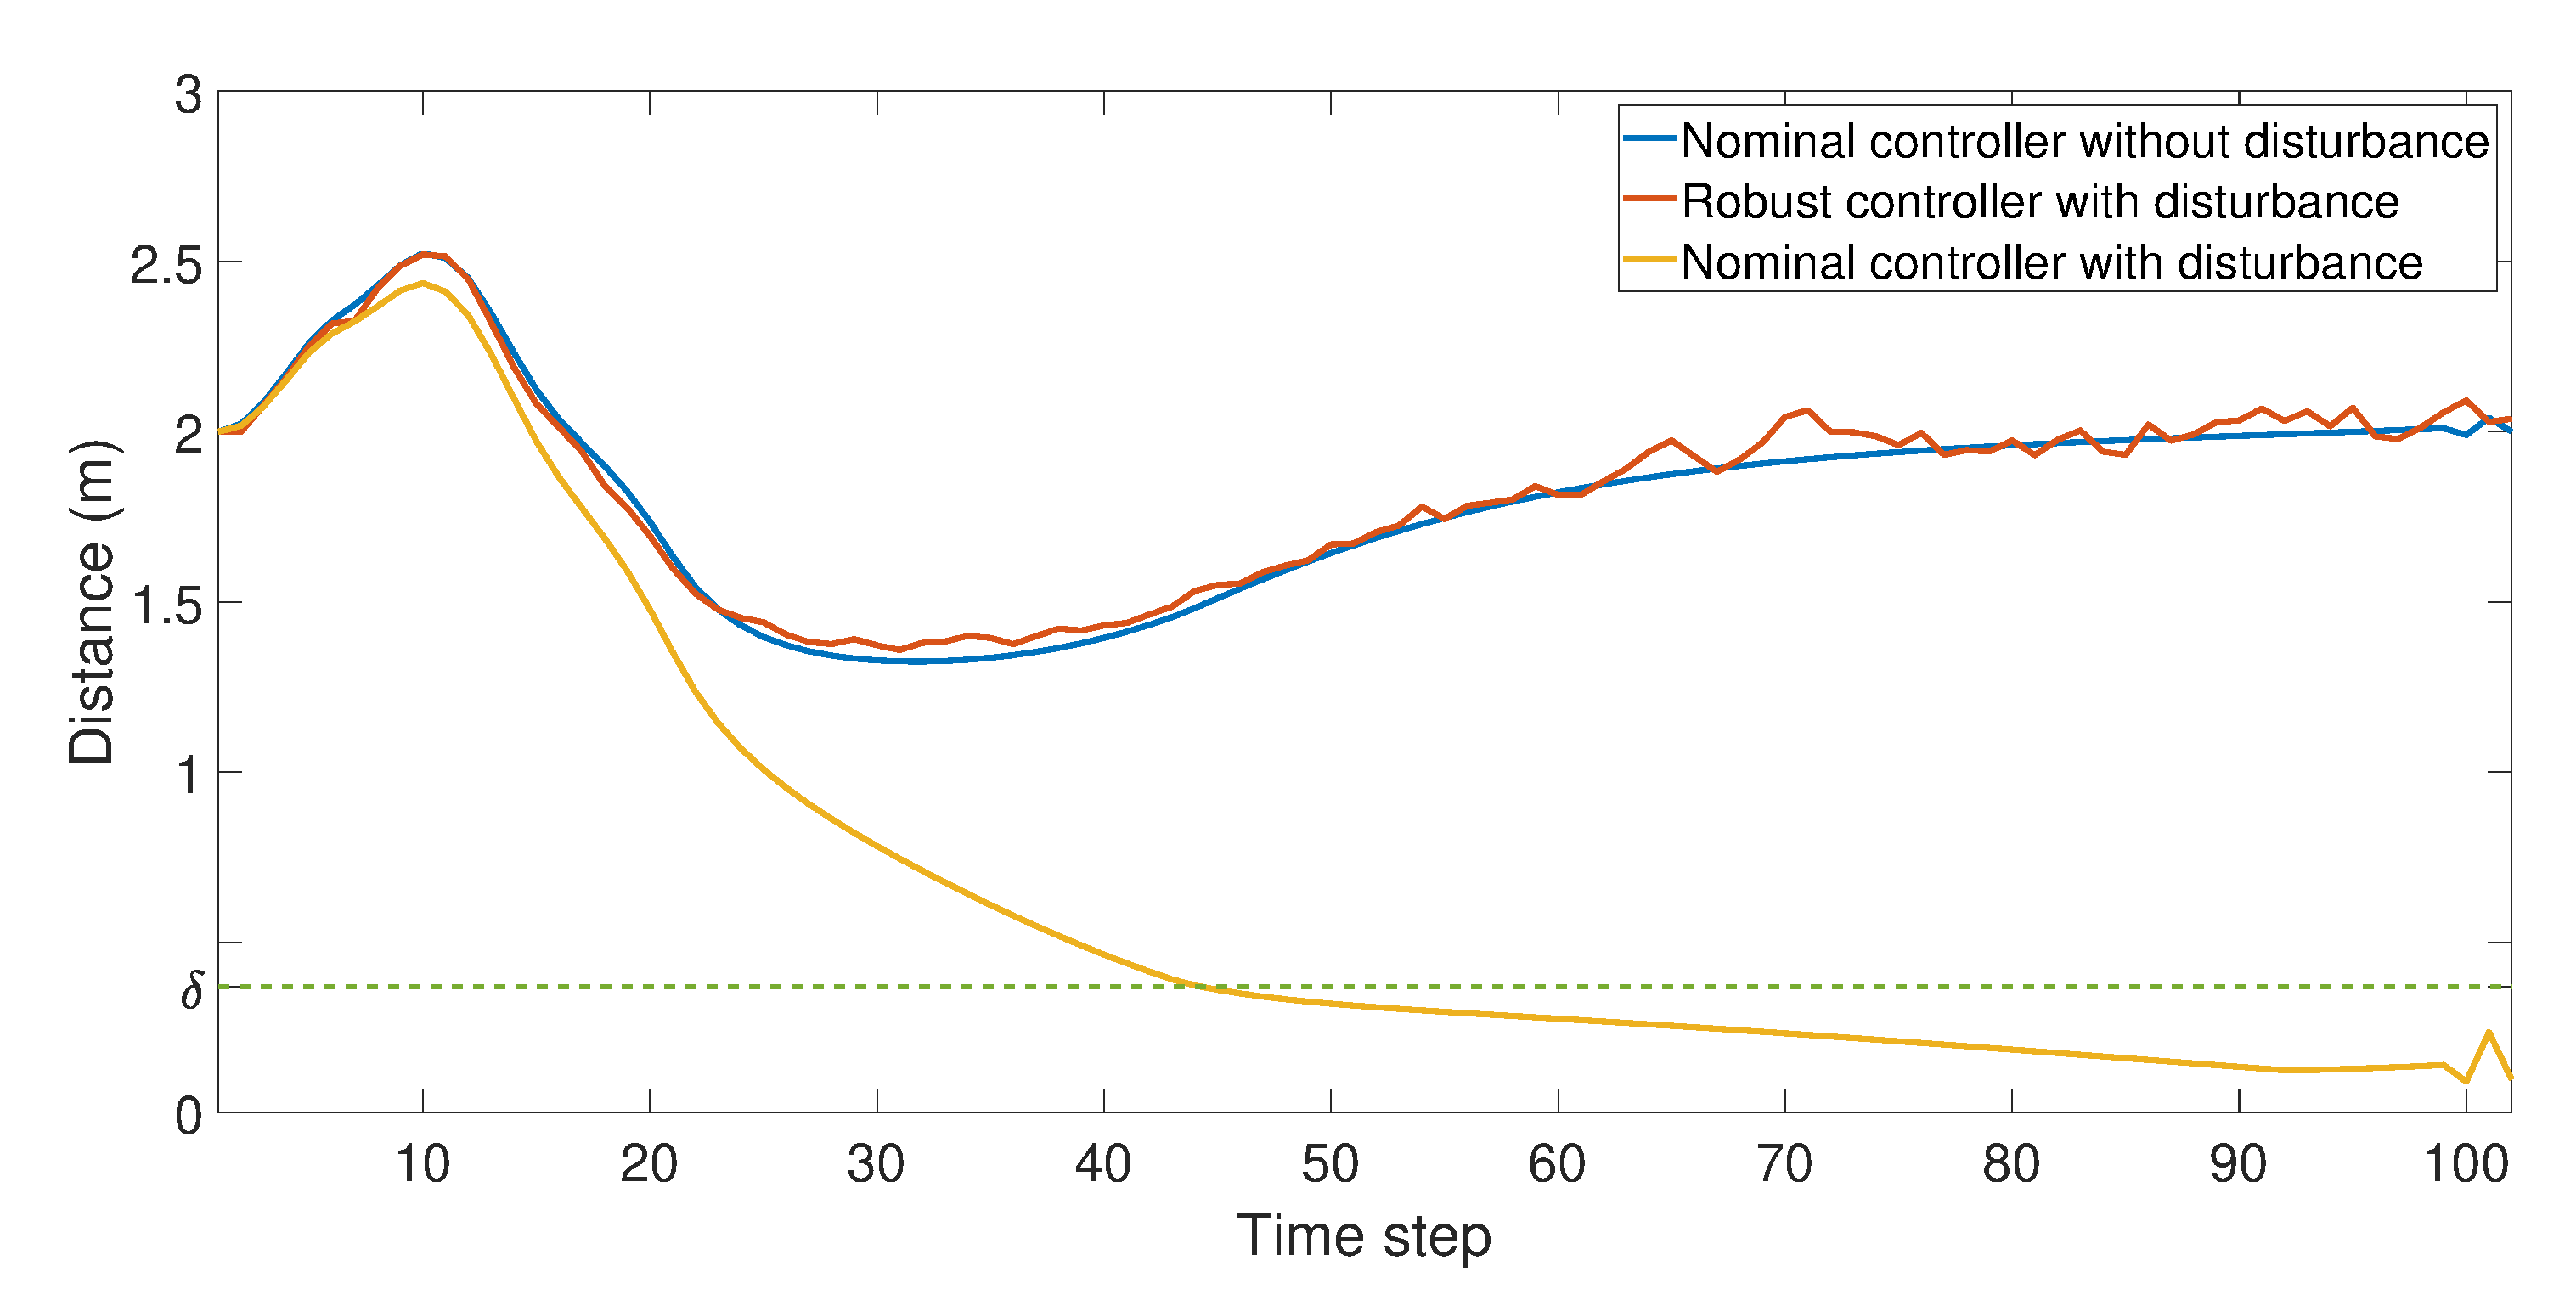
\includegraphics[width=.4\textwidth]{figures/multi_drone2.eps}
	\caption{Performance of open-loop and feedback controllers in regulating distance between two selected drones for disturbance-free and perturbed situations for the multi-drone path planning example}
	\label{fig:multi_drone_distance}
\end{figure}

\subsection{Crane and Vehicle}
\label{subsec:crane_vehicle}
We model the crane and vehicle as control systems 
$\Sigma^1=(X^1,x_\init^1,U^1,W^1,f_\tau^c)$ and $\Sigma^2=(X^2,x_\init^2,U^2,W^2,f_\tau^l)$, respectively.
The dynamics are obtained by discretizing the following continuous-time dynamics.

The crane is modeled as cart-pole system \cite{Barto1983}:
\begin{align*}
	\ddot{\theta} &= \frac{M_tg\sin(\theta) - \cos(\theta)(F + M_pl \dot{\theta}^2 \sin(\theta))}{l(4/3 M_t- M_p \cos^2(\theta))}=f^c_1(\theta,\dot{\theta},F)\\
	\ddot{z}&= \frac{F + M_pl \dot{\theta}^2 \sin(\theta)-M_pl \ddot{\theta} \cos(\theta)}{M_t}=f^c_2(\theta,\dot{\theta},F),
\end{align*}
where
	$g=-9.8$ m/s$^2$ is the acceleration of gravity,
	$M_c=1$ kg is the cart mass,
	$M_p=0.1$ kg is the pole mass,
	$M_t=M_c+M_p$ denotes the total mass,
and
	$l=0.5$ m is the half-pole length.
Further, the cart's position, the pole's angle, and input force to the cart are denoted by $x_1^{(1)}=z$ (in $m$), $x_3^{(1)}=\theta$ (in $Radian$), 
and $u^{(1)}=F$ (in $kg *m/s^2$), respectively. 
The continuous-time dynamics of the crane is of the following form:
\[f^{c}(x^{(1)}(t),u^{(1)}(t)):=\begin{bmatrix}
	\dot{x}_1^{(1)}\\
	\dot{x}_2^{(1)}\\
	\dot{x}_3^{(1)}\\
	\dot{x}_4^{(1)}
\end{bmatrix}=\begin{bmatrix}
\dot{z}\\
\ddot{z}\\
\dot{\theta}\\
\ddot{\theta}
\end{bmatrix}=
\begin{bmatrix}
	x_2^{(1)}\\
	f^c_1(x_3^{(1)},x_4^{(1)},u^{(1)})\\
	x_4^{(1)}\\
	f^c_2(x_3^{(1)},x_4^{(1)},u^{(1)})\\
\end{bmatrix}.\]
%with
%\begin{align}
%	f^c_2(x{(1)},u^{(1)})=\frac{g\;\sin(x_3^{(1)})}{}
%\end{align}
%\MS{what are $f^c_1$ and $f^c_2$?}
%The output mapping for the crane is defined as
%\[
%h^c(x^{(1)}(t))=\begin{bmatrix}
%	x_1^{(1)}+l \sin(x_3^{(1)})\\
%	y_1+l \cos(x_3^{(1)})
%\end{bmatrix},
%\]
%where, $y_1>0$ is a constant that denotes the cart's height from the ground.
The vehicle's continuous-time dynamics takes the form of
\[f^{l}(x^{(2)}(t),u^{(2)}(t))=\begin{bmatrix}
\dot{x}_1^{(2)}\\ \dot{x}^{(2)}_2 \end{bmatrix}=\begin{bmatrix} x^{(2)}_2\\ u^{(2)} \end{bmatrix},
\]
where $x_1^{(2)}$ and $x_2^{(2)}$ denote the vehicle's position in $m$ and speed in $m/s$ and $u^{(2)}$ represents the vehicle's control input (acceleration). 
On fixing the sampling time $\tau=0.1s$, one can derive $f^c_\tau$ and $f^l_\tau$. For the crane, the disturbance set and robustness margin are chosen as $|W^1|\leq(0,0.05,0,0)$ and  $\varepsilon^{1}=(0.135,0.385,0.176 ,0.768)$. Similarly, for the vehicle, disturbance set and robustness margin are chosen as $|W^2|\leq(0,0.1)$ and $\varepsilon^{2}=(0.08,0.12)$.
%The output mapping for the crane is defined as
%\[
%h^l=\begin{bmatrix}
%	x_1^{(2)}\\
%	y_2
%\end{bmatrix},
%\]
%where, $y_2>0$ is a constant that denotes the height of the forklift's head with respect to the ground.

There is no obstacle for this example and for minimum distance between the crane and the vehicle we choose $\delta=0.035$.
Fixing the horizon length to $T=70$, ALTRO was capable of generating a valid nominal trajectory in $0.65$ seconds. 
Fig.~\ref{fig:cr_and_lft} (\textbf{left}) demonstrates snapshots of the produced trajectory. 
As before, under the nominal open-loop controllers, applying (constant) additive disturbance $W=(0,0.05,0,0)$ (to the cart-pole system) 
causes a collision between the crane and the vehicle before the end of the mission (Fig.~\ref{fig:cr_and_lft} (\textbf{right})).

In the next step, we use SCOTS in order to compute a feedback controller tolerating disturbances $W^1$ and $W^2$. 
We choose state and input spaces for the crane to be $X^{1}=[-0.195,5.49]\times[-1.99,4.37]\times[1.20,4.68]\times[-5.44,5.28]$ and $U^{1}=[-7,7]$, respectively. For the vehicle, we set $X^{2}=[3,9]\times[-3,1.995]$ and $U^{2}=[-3,3]$. %Next, we augment both dynamics with time and 
We choose state and input partition sizes $\eta_{{X}}^{1}=(0.015,0.035,0.016,0.064)$, $\eta_{U}^1=0.2$,  $\eta_{{X}}^2=(0.01,0.015)$ and $\eta_{U}^2=0.1$. %These selections yield discretized models with state and input spaces having $2.5\times 10^9$ and $71$ points for the crane, and $2\times 10^5$ and $61$ points for the vehicle. 
%Next, we limit both of the state spaces into tubes constructed around the open-loop trajectories with sizes specified as $\varepsilon^{1}=\begin{bmatrix}0.135&0.385&0.176 &0.768\end{bmatrix}^T$ and $\varepsilon^{2}=\begin{bmatrix}0.08&0.12\end{bmatrix}$. %This reduces size of state spaces into $1.2\times 10^7$ and $1.5\times 10^4$ for the crane and vehicle, respectively. 
%Given the above settings, SCOTS was able to compute abstraction in $511$ and $0.22$ seconds for the crane and the vehicle, respectively. Scots performs synthesis in $91$ and $0.037$ seconds for the crane and the vehicle, respectively.
Tab.~\ref{tab:runtimes} shows the run times and number of state-input pairs corresponding to local and global ABCD. 
As before, for the cart-pole model, global ABCD exceeds our 1.5TB  memory limit. 
Note that computing feedback controllers for the crane and vehicle takes 511 seconds and 0.3 seconds, respectively. 
The large difference is due to the difference in the size of transition systems for the two dynamics. 
% \RM{we said the following already:}
% As mentioned before, using ALTRO alone would not provide guarantee against bounded disturbance (Fig~\ref{fig:cr_and_lft}, \textbf{right}). 

			
%\begin{figure}[t]
%	\centering
%	\includegraphics[width=0.45\textwidth]{figures/crane_and_forklifter.pdf}
%	\caption{Illustration of the trajectories generated by the open-loop controller for the crane and vehicle example under disturbance-free (\textbf{left}) and perturbed (\textbf{right}) situations} 
%	\label{fig:cr_and_lft_2}
%\end{figure}


%In this example, we show the method can handle multiple heterogeneous dynamical systems. This example is Modelling a special situation in a factory(shown in fig \ref{fig:cr_and_lft}) . Assume there is a crane and and a forklift. Each one of them should reach their destination without having any accident(satisfying specs). The Crane position will change from 0 to 5 and the forklift from 9 to 4.  Here we model the forklift using $\begin{bmatrix} \dot{x_1}\\ \dot{x_2} \end{bmatrix}=\begin{bmatrix} x_2\\ u \end{bmatrix}$ ($x_1$ and $x_2$ are representing position and velocity) and for the crane we use inverted pendulum model with exactly same configuration in \cite{barto1983neuronlike}: \\ 
%\[\begin{bmatrix}
%\dot{x}\\
%\Ddot{x}\\
%\dot{\theta}\\
%\Ddot{\theta}
%\end{bmatrix}=\begin{bmatrix}
%\dot{x_1}\\
%\dot{x_2}\\
%\dot{x_3}\\
%\dot{x_4}
%\end{bmatrix}=\begin{bmatrix}
%x_2\\
%g(x_3,x_4,u)\\
%x_4\\
%f(x_3,x_4,u)\\
%\end{bmatrix}\]
%
%where $x$ represent position of the cart  and $\theta$ is angle of the pole, f and g are non-linear functions. The process of controller design is similar to Sec. \ref{sec:MultiAgent}; At first we find a nominal trajectory with ALTRO with required specifications then we robustifing it using our method with modified ABCD.\\
%In this example we do not have any static obstacle, but for collision avoidance we use euclidean distance as the metric with $\delta=0.4$ for measuring distance between crane and forklift. We consider hook of crane as a point mass with a radius and forklift as several point mass on circumference of it, So we consider minimum distance between the hook and points of the forklift as the distance. ALTRO solve this trajectory generation problem using sampling time =0.1 and number of points=40 in 10.7 seconds.\\
%to guarantee collision avoidance specification we should select tube sizes to satisfy:
%\[ \delta_{col}> \varepsilon_x + l*\varepsilon_\theta + \varepsilon^\prime_x\]
%where $\varepsilon_x$ and $\varepsilon_\theta$ are tube sizes for position and angle in crane model (cart pole) and l is the length of the joint and $\varepsilon^\prime_x$ is tube size for position of the forklift.
%In next phase we use finite abstraction with $\varepsilon_x=9*0.015$ and $\varepsilon_\theta=11*0.015$ and $\varepsilon^\prime_x=9*0.015$. It takes about 1000 seconds for crane (cart-pole system) with (1.15)*($10^{11}$) number of state-input pairs and ($7*10^6$)*(71) reduced number of states and synthesis takes 35 seconds. For forklift abstractions abstraction and synthesis will finish in less than a second.\\
%The nominal controller with disturbances $w_1=[0,0.02,0,0]$ for crane and $w_2=[0,0.1]$ for forklift will fail collision specification.
%
%


%} 

\begin{figure}
	\centering
	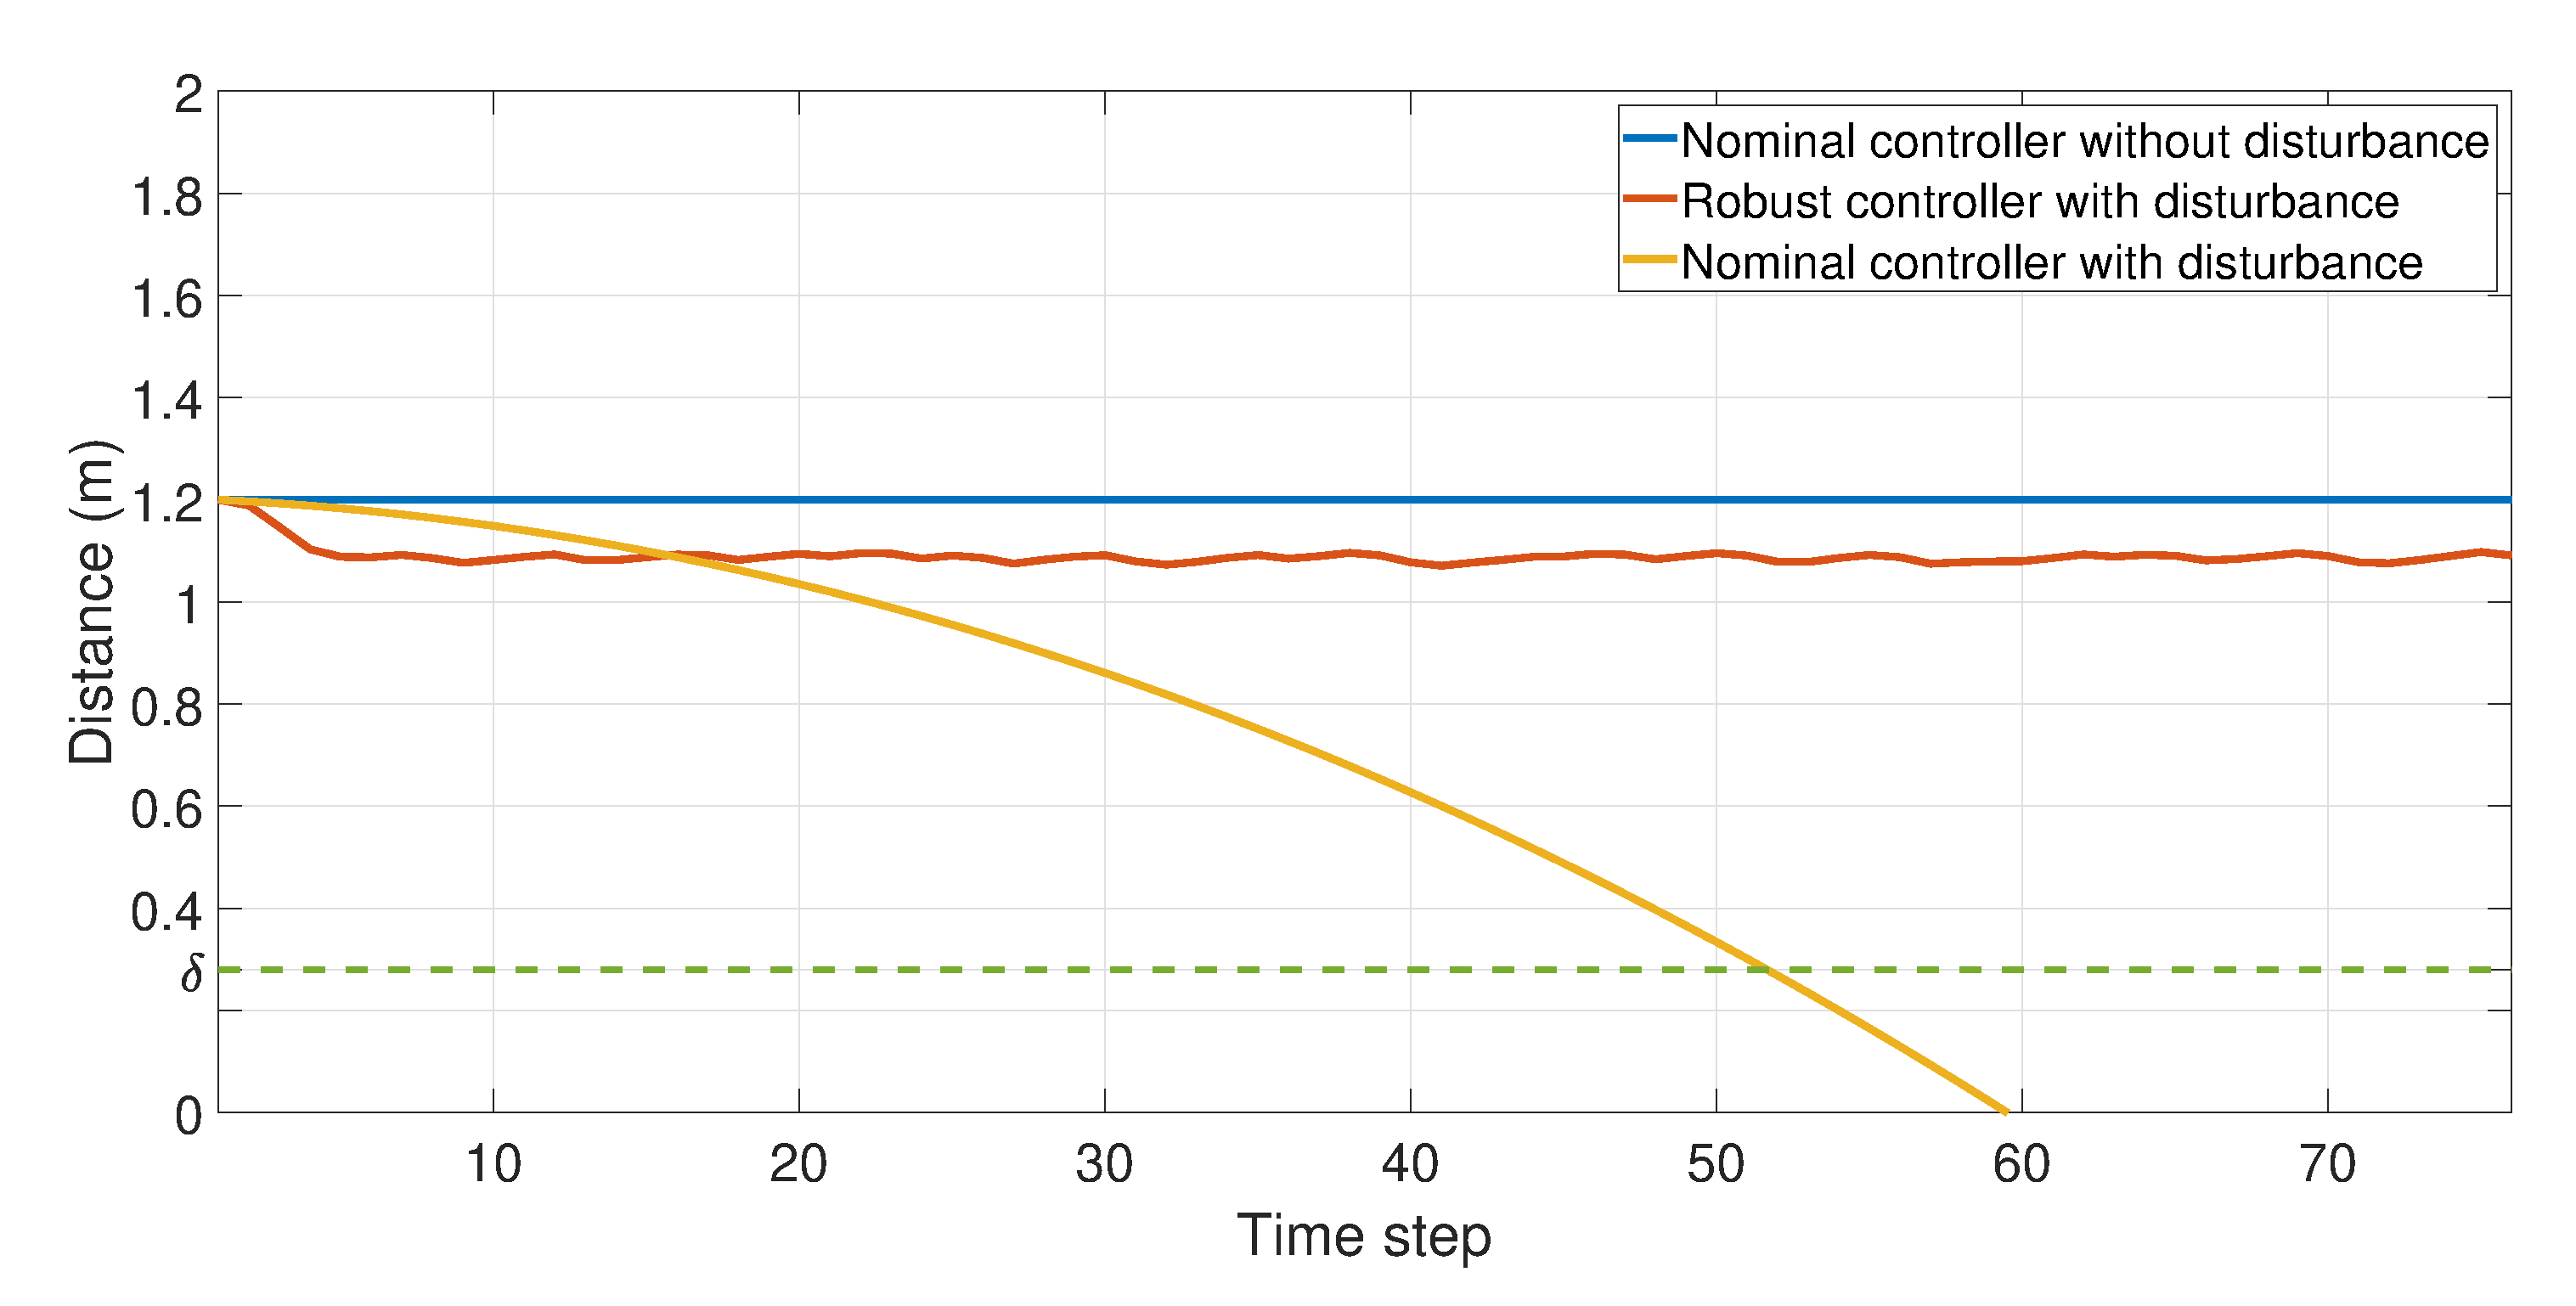
\includegraphics[width=0.45\textwidth]{figures/Merge_plot2.eps}
	\caption{Comparison of open-loop and feedback controllers for the lane merging example}
	\label{fig:merging_distance}
	\vspace*{-0.3cm}
\end{figure}

\subsection{Lane Merging}
\label{sec:lane merging}

%Every vehicle is modeled as tuple $\Sigma=(X,U,W,f^v,Y,h^v)$. 
%Dynamics for each vehicle takes the form
%\begin{equation*}\label{eq:vehicle_ss}
%	f^{v}(x(t),u(t))=
%	\begin{bmatrix}
%		\dot{x_1}\\
%		\dot{x_2}
%	\end{bmatrix}=
%	\begin{bmatrix}
%		u_1\\
%		u_2
%	\end{bmatrix},
%\end{equation*}
%where $x_1$, $x_2$ denote the vehicle's position in $2D$ plane, $u_1$ and $u_2$ represent the vehicle's speed coordinates, respectively. The output mapping is defined as
%\[
%h^v(x(t))=x(t).
%\]
The nominal dynamics for each of the vehicles is the same as the one  for modeling drones (given in Sec.~\ref{sec:Multirobot}). 
The disturbance set and robustness margin are chosen as $|W|\leq (0.03,0.03,0.03)$ and $\varepsilon=(0.16,0.16,0.16)$. %($\Sigma^i=(X,x_\init^i,U,W,f^d_\tau)$). 
For collision and obstacle avoidance, we choose $\delta=0.37$.
The horizon length is fixed to $T=110$. 
Given these settings, ALTRO generates a valid nominal trajectory in $89.02$ seconds. 
Next, we use ABCD in order to compute feedback controllers tolerating additive disturbance $W$. 
We choose state and input spaces for each vehicle's model to be $X=[-0.5,15]\times[0.1,7.4]\times[-1,0.4]$ and $U=[-0.9,3]\times[-2.1,2.1]$, respectively. 
State and input partition sizes are chosen as $\eta_{X}=(0.02,0.02,0.02)$ and $\eta_{U}=(0.3,0.15)$. 
Tab.~\ref{tab:runtimes} shows run times and number of state-input pairs corresponding to local and global ABCD. 
For $N>1$, memory requirement for global ABCD exceeds memory limits.
Fig.~\ref{fig:merge} demonstrates snapshots of one sample trajectory when feedback controllers are employed under the presence of disturbance. It should be noticed that using ALTRO alone would not provide guarantee against bounded disturbance.
Fig.~\ref{fig:merging_distance} illustrates the fact that open-loop controller fails in keeping one of the vehicles away from the road's sides under perturbed situation when constant additive disturbance vector $(-0.03 ,0.03,-0.03)$ is being applied throughout the whole horizon. 
In contrast, employing a feedback controller results in successful lane merging. 





\begin{figure}[t]
	\centering
	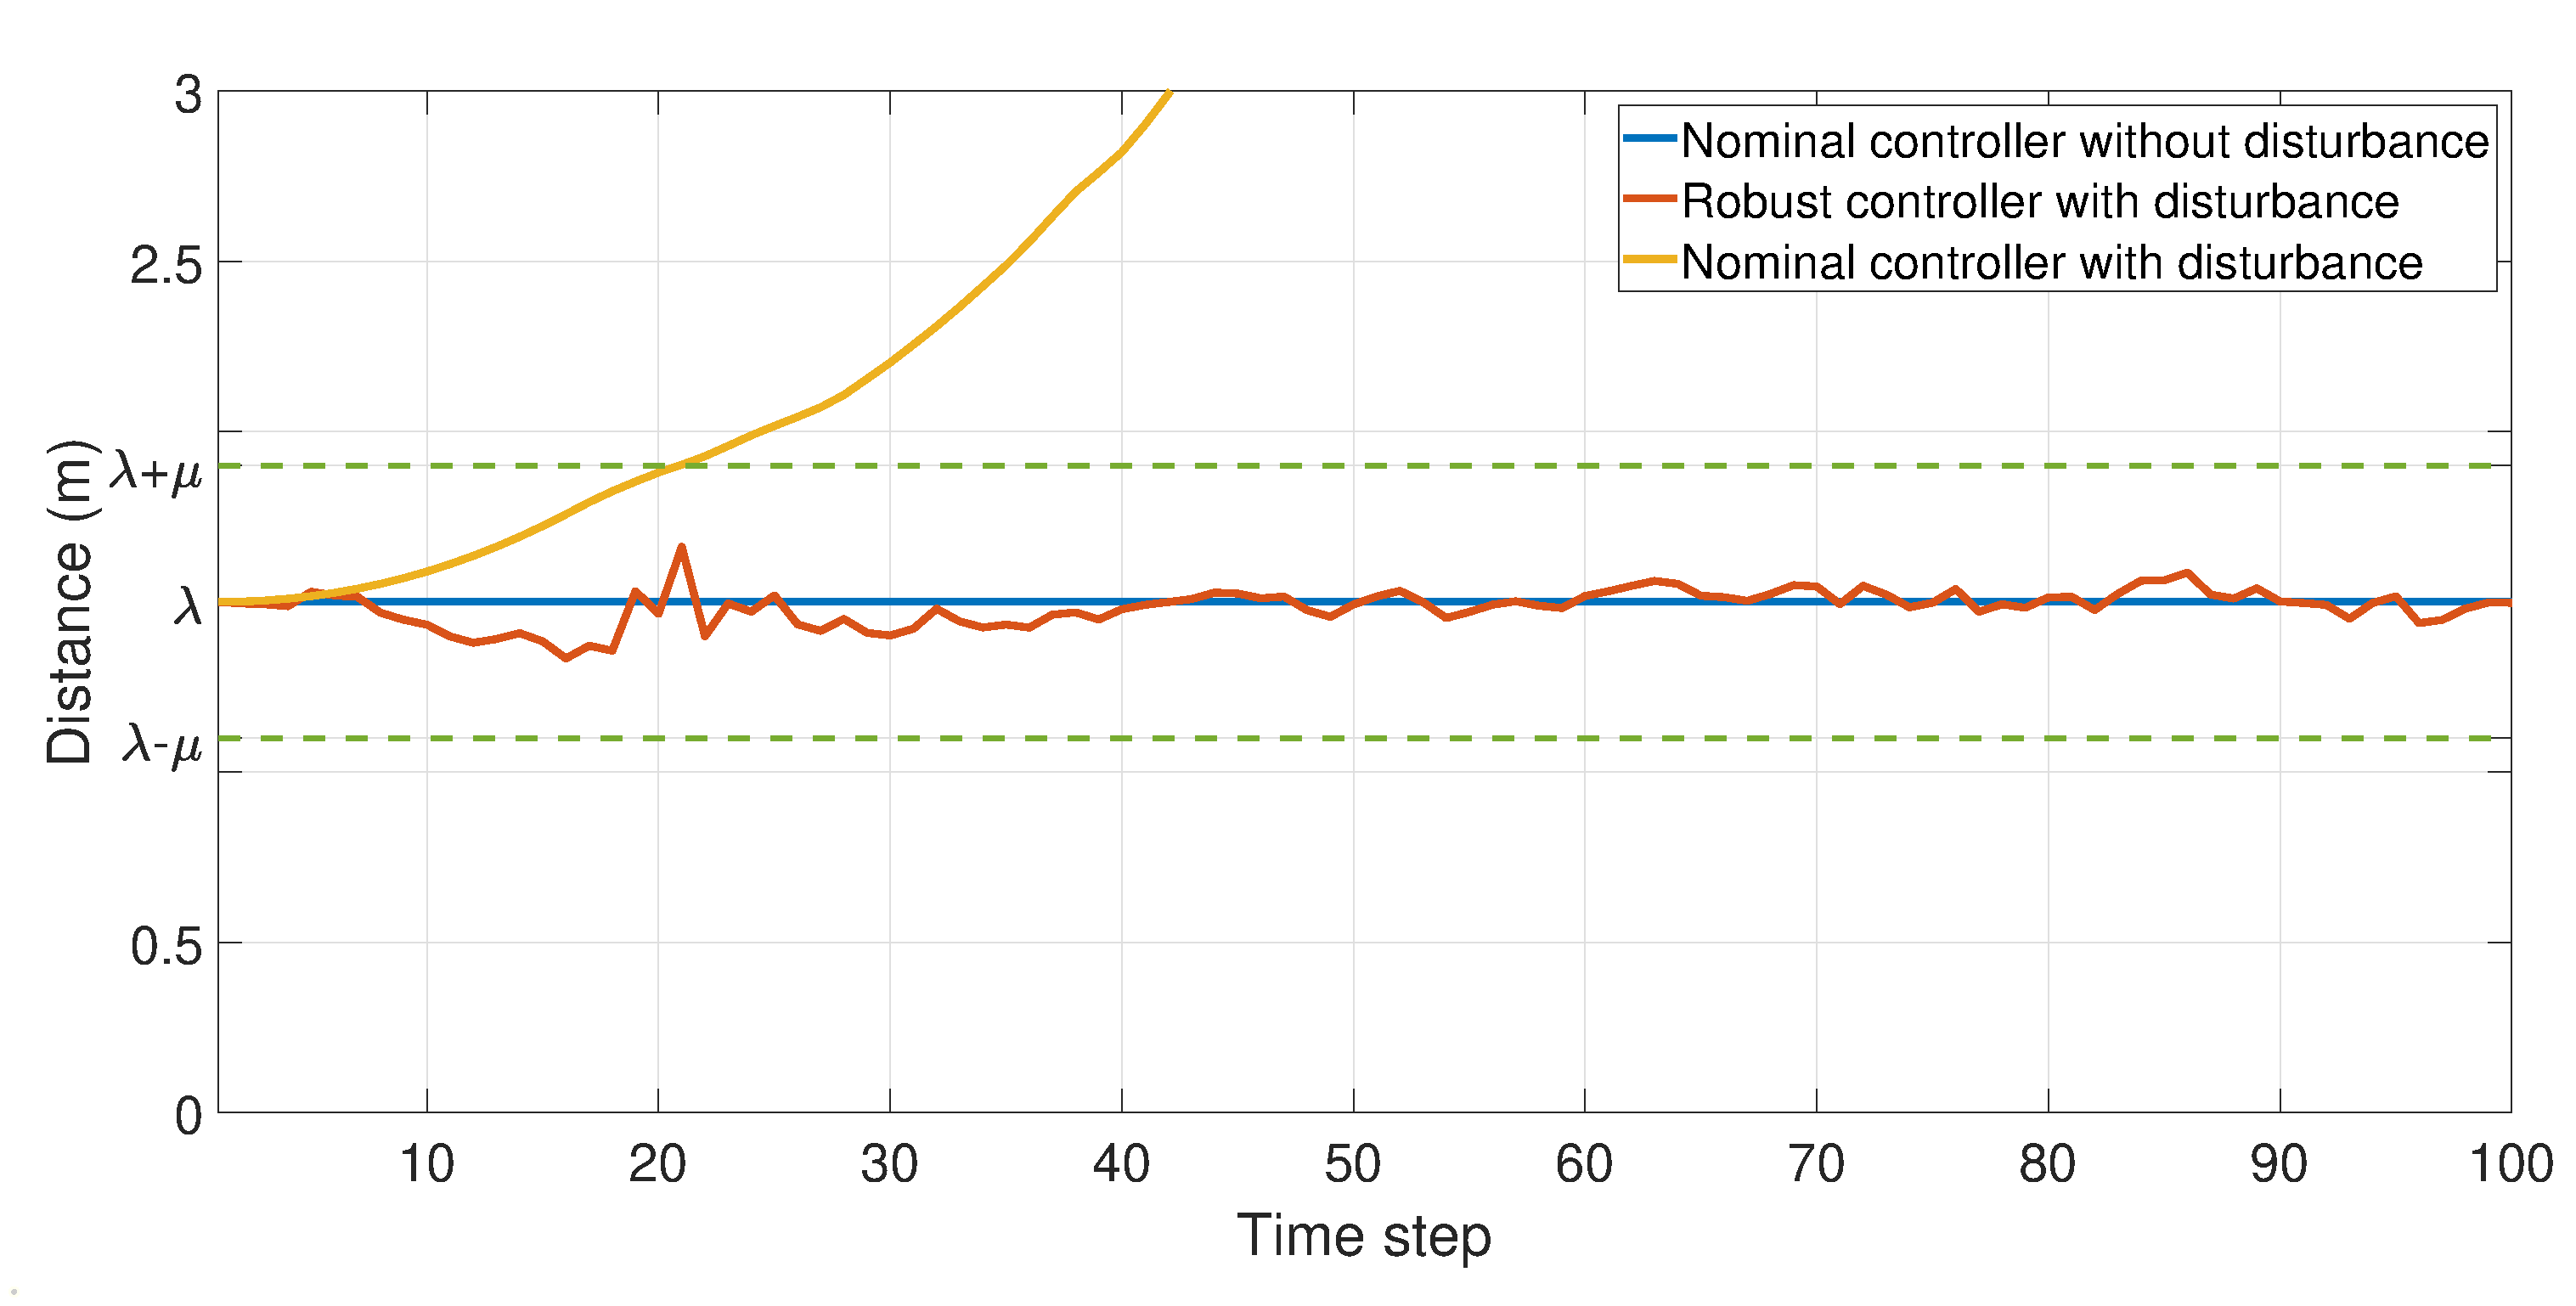
\includegraphics[width=0.45\textwidth]{figures/formation_dist2.eps}
	\caption{Comparison of open-loop and feedback controllers for the formation control example}
	\label{fig:formation_distance}
	\vspace*{-0.5cm}
\end{figure}

\subsection{Multi-drone formation control}
\label{sec:formation_control}

In the multi-drone formation control case study, the nominal dynamics for each of the drones is the same as that in 
Sec.~\ref{sec:Multirobot}. 
The disturbance set and robustness margin are chosen as $|W|\leq (0.03,0.03,0.03)$ and $\varepsilon=(0.24,0.24,0.24)$. 
Distance between each pair of drones positioned at the diamond's vertices is set to be $\lambda^{i,j}=\frac{3\sqrt{2}}{2}$ 
for $i,j\in\set{1,2,3,4}$, while the drone positioned at the center is supposed to keep distance $\lambda^{5,j}=1.5$ 
for $j\in\set{1,2,3,4}$. 
Setting the minimum distance for obstacle avoidance to $\delta=0.4$ and horizon length $T=100$, 
ALTRO finds a valid solution over the product system with $15$ state and $10$ input variables within $114.3$ seconds.
Next, we synthesize local controllers for every drone such that the specifications hold for the perturbed models with $\mu=0.5$. %We construct a tube around the (nominal) trajectory produced by ALTRO with the width vector $\varepsilon=\begin{bmatrix}??&??&??\end{bmatrix}^T$.
%\RM{the state space should go before ALTRO}
We consider state and input spaces to be $X=[-2,17]\times[-2,17]\times[0.6,1.6]$ and
$U=[-0.9,4.8]\times[-3,3]$, respectively. We select $\eta_{X}=(0.03,0.03,0.03)$ and
$\eta_{U}=(0.3,0.15)$. % and $\varepsilon=\begin{bmatrix}0.18&0.18&0.18\end{bmatrix}^T$.% results in state and input spaces with $10^9$ and $820$ points. 
%Computing the transition system over inter-tube space with width $\varepsilon=\begin{bmatrix}0.18&0.18&0.18\end{bmatrix}^T$ results in smaller transition system with $4.9\times 10^5$ points. Given the above settings, SCOTS computes abstraction in $271$ seconds ($54.2$ seconds in average) and $66.5$ seconds ($13.3$ seconds in average). 
Tab.~\ref{tab:runtimes} shows the run times and number of state-input pairs corresponding to local and global ABCD. 
Already for two drones, the memory requirement for global ABCD exceeds the available memory of 1.5TB of RAM.
Fig.~\ref{fig:formation_ex} illustrates four sequential frames of a sample perturbed trajectory generated by employing 
feedback controllers. Notice that both 
relative position and orientation between drones are kept (almost) constant 
throughout the journey. 
On the other hand, using ALTRO alone would not provide guarantee against bounded disturbance. 
Fig.~\ref{fig:formation_distance} illustrates performance of open-loop and feedback controllers on regulating distance between two specific 
drones with and without disturbances. 
As expected, in the absence of disturbances, the open-loop controllers suffice and the distance between the two drones 
(shown in solid blue) does not go below the threshold line (showed as the dotted line). 
However, when constant additive disturbance vectors 
$(0 ,0.03,0.03)$ and $(0 ,-0.03,-0.03)$
are being applied to the two drones throughout the whole horizon, open-loop controller fails, 
whereas the feedback controller is still capable of maintaining distance above the given threshold.


\end{appendix}

\end{document}
